%%%%%%%%%%%%%%%%%%%%%%%%%%%%%%%%%%%%%%%%%%%%%%%%%%%%%%%%%%%%%%%%%%%%%%%%%%%%
%% Author template for Operations Reseacrh (opre) for articles with no e-companion (EC)
%% Mirko Janc, Ph.D., INFORMS, mirko.janc@informs.org
%% ver. 0.95, December 2010
%%%%%%%%%%%%%%%%%%%%%%%%%%%%%%%%%%%%%%%%%%%%%%%%%%%%%%%%%%%%%%%%%%%%%%%%%%%%
\documentclass[fleqn,mnsc,nonblindrev]{informs4}
%%\documentclass[opre,nonblindrev]{informs3_modified} % current default for manuscript submission

\usepackage{fix-cm}
\makeatletter
\long\def\@makefigurecaption#1#2{\EGT\FigureCaptionFontStyle
\FigureNameFontStyle #1\ \ignorespaces #2\HD{0}{9}\endgraf}
\makeatother
\makeatletter
\long\def\@maketablecaption#1#2{\EGT\TableCaptionFontStyle
\noindent\textbf{#1} #2\par}
\makeatother

%%%%%%%%%%% Other packages
\usepackage{booktabs}
\usepackage{subcaption}
\captionsetup[sub]{font=small,labelfont={bf,sf}}
\usepackage{pgfplots}
\usepgfplotslibrary{fillbetween}
\pgfplotsset{compat=1.18}
\usepackage{adjustbox}

% Commands---------------------------------------
\newcommand{\ex}[1]{\mathbb{E}\left[#1\right]}
\newcommand{\ttr}[1]{\textcolor{red}{#1}}
\newcommand{\ttb}[1]{\textcolor{blue}{#1}}
\newcommand{\Normal}{\operatorname{Normal}}
\newcommand{\CE}{\operatorname{CE}}
\newcommand{\EE}{\mathbb{E}}
\newcommand{\QQ}{\mathbb{Q}}
\newcommand{\PP}{\mathbb{P}}
\newcommand{\Var}{\operatorname{Var}}
\newcommand{\Cov}{\operatorname{Cov}}
\newcommand{\var}[2]{\mathrm{VaR}_{#1}(#2)}
\newcommand{\indi}[1]{\mathbb{I}_{\{#1\}}}
\newcommand{\prob}[1]{\mathbb{P}[#1]}
\newcommand{\ifn}[1]{\mathbbm{1}_{\{#1\}}}
\newcommand{\ig}[4]{\int_{#1}^{#2}\,#3\,\mathrm{d}{#4}}
\newcommand{\tvar}[2]{\mathrm{TVaR}_{#1}(#2)}
\newcommand{\com}[1]{{ \color{red} [#1] }}
\newcommand{\tb}[1]{\textbf{#1}}
\definecolor{darkpastelgreen}{rgb}{0.01, 0.75, 0.24}
\newcommand{\blfootnote}[1]{
\begingroup
\renewcommand\thefootnote{}\footnote{#1}
\addtocounter{footnote}{-1}
\endgroup
}
\newcommand{\eg}{\textit{e.g.}}
\newcommand{\ie}{\textit{i.e.}}
\renewcommand{\Re}{\mathbb{R}}

% Line Spacing
\OneAndAHalfSpacedXI

% figure packages
\usepackage{graphicx}
% \usepackage{eqndefns-left}
\usepackage{multirow}
\usepackage{hhline}

% caption package
% \usepackage[small, margin=1cm]{caption}
\usepackage[font=small, margin=1cm]{caption}

% color packages
\usepackage{color}
\definecolor{strcolor}{rgb}{0.6, 0.2, 0.6}
\definecolor{commentcolor}{rgb}{0.3125, 0.5, 0.3125}
\definecolor{keycol}{rgb}{0, 0, 1}

% revision
\newcommand{\rev}[1]{{\color{red} #1}}

% math packages
\usepackage{amssymb}
\usepackage{amsmath}
\usepackage{bbm}

% hyperlinks packages
\usepackage{hyperref}
\usepackage{url}

% Equation environments
\newcommand {\bea}{\begin{eqnarray}}
\newcommand {\eea}{\end{eqnarray}}
\newcommand {\E}[1]{\mathrm{E}\left( #1 \right)}
\newcommand {\Ep}[2]{{\mathrm{E}_{\mathbb{P}_{#1}} \left( #2 \right)}}
\newcommand {\supEp}[1]{\displaystyle \sup_{\mathbb{P} \in \mathbb{F}} \Ep{}{#1}}
\newcommand {\supEpf}[2]{\displaystyle \sup_{\mathbb{P} \in \mathbb{F}_{#1}} \Ep{}{#2}}
\newcommand {\pos}[1]{\paren{#1}^+}
\renewcommand {\neg}[1]{\paren{#1}^-}
\newcommand {\pibound}[1]{\ensuremath{\pi^{#1}\paren{r^0, \mb{r}}}}
\newcommand {\etabound}[1]{\ensuremath{\eta^{#1}\paren{r^0, \mb{r}}}}
\newcommand \conv {\mathrm{conv}}
\newcommand {\p}{{\rm P}}
% mb
\newcommand{\mb}[1]{\mbox{\boldmath \ensuremath{#1}}}
\newcommand{\mbt}[1]{\mb{\tilde{#1}}}
\newcommand{\mbb}[1]{\mb{\bar{#1}}}
\newcommand{\mbbs}[1]{\mbb{\scriptstyle{#1}}}
\newcommand{\mbh}[1]{\mb{\hat{#1}}}
\newcommand{\mbth}[1]{\mbt{\hat{#1}}}
\newcommand{\mbc}[1]{\mb{\check{#1}}}
\newcommand{\mbtc}[1]{\mbt{\check{#1}}}
\newcommand{\mbs}[1]{\mb{\scriptstyle{#1}}}
\newcommand{\mbst}[1]{\mbs{\tilde{#1}}}
\newcommand{\mbsh}[1]{\mbs{\hat{#1}}}
% mc
%\newcommand{\mc}[1]{\mbox{\ensuremath{\mathcal{#1}}}}
\newcommand{\mch}[1]{\hat{\mc{#1}}}
\newcommand{\mcs}[1]{\mc{\scriptstyle{#1}}}
\newcommand{\mcss}[1]{\mc{\scriptscriptstyle{#1}}}
\newcommand{\mcsh}[1]{\hat{\mcs{#1}}}
\newcommand{\mbss}[1]{{\mbox{\boldmath \tiny{$#1$}}}}
\newcommand{\eucnorm}[1]{\left\| #1 \right\|_2}
\newcommand{\dpv}{\displaystyle \vspace{3pt}}
\newcommand{\diag}[1]{\textbf{diag}\paren{#1}}
\newcommand{\yldrk}{\mb{y}^k\paren{\mbt{z}}}
\newcommand{\abs}[1]{\left| #1 \right|}
\DeclareMathOperator{\CVaR}{CVaR}
\DeclareMathOperator{\VaR}{VaR}
%\DeclareMathOperator{\argmin}{\arg\min}
% combinations
\renewcommand{\mbc}[1]{\mb{\mc{#1}}}
%misc
\newcommand{\ceil}[1]{\left\lceil #1  \right\rceil}

%\newtheorem{theorem}{Theorem}
%\newtheorem{lemma}[theorem]{Lemma}
\newtheorem{conj}{Conjecture}
\newtheorem{coro}{Corollary}
%\newtheorem{claim}{Claim}
\newtheorem{Defi}{Definition}
\newtheorem{algorithm}{Algorithm}
%\newtheorem{assumption}{Assumption}
%\renewcommand{\bigtimes}{\mathop{\rm \text{\Large{$\times$}}}}

\def\blot{\quad \mbox{$\vcenter{ \vbox{ \hrule height.4pt
\hbox{\vrule width.4pt height.9ex \kern.9ex \vrule width.4pt}
\hrule height.4pt}}$}}

% Natbib setup for author-year style
\usepackage{natbib}
\bibpunct[, ]{(}{)}{,}{a}{}{,}%
\def\bibfont{\fontsize{8}{9.5}\selectfont}%
\def\bibsep{0pt}%
\def\bibhang{16pt}%
\def\newblock{\ }%
\def\BIBand{and}%
\bibliographystyle{plainnat}

%% Setup of theorem styles. Outcomment only one.
%% Preferred default is the first option.
\TheoremsNumberedThrough     % Preferred (Theorem 1, Lemma 1, Theorem 2)
% \TheoremsNumberedByChapter  % (Theorem 1.1, Lema 1.1, Theorem 1.2)
\ECRepeatTheorems

%% Setup of the equation numbering system. Outcomment only one.
%% Preferred default is the first option.
\EquationsNumberedThrough    % Default: (1), (2), ...
% \EquationsNumberedBySection % (1.1), (1.2), ...

% In the reviewing and copyediting stage enter the manuscript number.
%\MANUSCRIPTNO{} % When the article is logged in and DOI assigned to it,
%   this manuscript number is no longer necessary

%\newdimen\setvrulersecondcolumnheightdimen%
%\newbox\setvrulersecondcolumnheightdimenbox%
%%%%%%%%%%%%%%%%%
\gdef\AQ#1{}
\gdef\CQ#1{}
%\setvruler [][1][1][1][1][5pt][5pt][0pt][\textheight]

\begin{document}

% \linenumbers

%%%%%%%%%%%%%%%%

%	\AIA
% \setcounter{page}{1} %
% \VOL{00}%
% \NO{0}%
% \MONTH{Xxxxx}%
% \YEAR{2017}%
% \FIRSTPAGE{1}%
% \LASTPAGE{16}%
% \FIRSTPAGEAIA{1}%
% \LASTPAGEAIA{16}%
\def\COPYRIGHTHOLDER{INFORMS}%
\def\COPYRIGHTYEAR{2017}%
\def\DOI{\fontsize{7.5}{9.5}\selectfont\sf\bfseries\noindent https://doi.org/10.1287/opre.2017.1714\CQ{Word count = 9740}}
%\def\RECEIVED{November 1, 2016}
%\def\REVISED{June 22, 2017; October 6, 2017}
%\def\ACCEPTED{November 15, 2017}
% \PUBONLINEAIA{}

\RUNAUTHOR{Anthropelos, Feng, and Kim} %

\RUNTITLE{On the Expansion of Risk Pooling}

\TITLE{On the Expansion of Risk Pooling}


% Block of authors and their affiliations starts here:
% NOTE: Authors with same affiliation, if the order of authors allows,
%   should be entered in ONE field, separated by a comma.
%   \EMAIL field can be repeated if more than one author

\ARTICLEAUTHORS{
\AUTHOR{Michail Anthropelos}
\AFF{Department of Banking \& Financial Management,
University of Piraeus}
\AUTHOR{Runhuan Feng}
\AFF{Department of Finance, School of Economics \& Management,
Tsinghua University}
\AUTHOR{Seongyoon Kim}
\AFF{Department of Mathematics, University of Illinois at Urbana-Champaign}
% \AUEXTRA{$^{*}$Corresponding author}
\AFFmail{{\bf Contact:} anthropel@unipi.gr, fengrh@sem.tsinghua.edu.cn, sk61@illinois.edu}%
}
% end of the block

% \ARTICLEINFO{\textbf{Received:} November 1, 2016\\ \textbf{Revised:} June 22, 2017; October 6, 2017\\ \textbf{Accepted:} November 15, 2017\\ \textbf{Published Online in Articles in Advance:}}

\ABSTRACT{Risk pooling has become an increasingly critical tool for managing risks among corporations, institutions, states, and nations, with examples including multinational pooling, decentralized insurance schemes, catastrophe risk pooling, and burden sharing for nuclear accidents. While there has been a rich literature on such practices, little is known from a theoretical viewpoint regarding the operational strategies of risk pools and in particular on issues about the effect of a pool's expansion on each existing member's welfare. This paper is the first to explore these issues by establishing different notions of consensus for the expansion of a risk pool: strong consensus, where both existing members and new candidates improve their risk measures due to the pool's expansion, and weak consensus, which refers to the willingness of existing members to remain in the pool. Under optimal risk sharing for each pool, we show that its properties regarding expansion's effects depend strongly on the underlying pricing rule. For instance, only with risk-adjusted equilibrium pricing are existing members willing to accept highly risky new members, whereas simple linear pricing excludes such members from the pool. Additionally, the impact of exogenous reinsurance on consensus is analyzed under both pricing rules. The established framework offers valuable managerial insights and policy implications, which we illustrate through two indicative case studies based on real data.}


%\FUNDING{The research of the first author is supported by NWO Grant 613.001.208. The third author acknowledges the funding support from the Singapore Ministry of Education Social Science Research Thematic Grant MOE2016-SSRTG-059.}

\SUBJECTCLASS{Decision analysis: risk}

\AREAOFREVIEW{Finance}

\KEYWORDS{risk sharing, risk pooling, decentralized insurance, catastrophe risk pooling, expansion}%{\CQ{Kindly provide the keywords.}}

%%%%%%%%%%%%%%%%%%%%%%%%%%%%%%%%%%%%%%%%%%%%%%%%%%%%%%%%%%%%%%%%%%%%%%

% Samples of sectioning (and labeling) in OPRE
% NOTE: (1) \section and \subsection do NOT end with a period
%       (2) \subsubsection and lower need end punctuation
%       (3) capitalization is as shown (title style).
%
%\section{Introduction.}\label{intro} %%1.
%\subsection{Duality and the Classical EOQ Problem.}\label{class-EOQ} %% 1.1.
%\subsection{Outline.}\label{outline1} %% 1.2.
%\subsubsection{Cyclic Schedules for the General Deterministic SMDP.}
%  \label{cyclic-schedules} %% 1.2.1
%\section{Problem Description.}\label{problemdescription} %% 2.
% Text of your paper here

\maketitle

\section{Introduction}
\subsection{Background}

Risk sharing is a risk management strategy employed across various industries to enhance welfare through the mutually beneficial transfer of risks. Over the past few decades, numerous forms of risk pooling have emerged in practice. These include insurers co-insuring parts of their portfolios, nations creating pools to share catastrophic risks, and financial institutions generating derivative securities to exchange exposures to different investment risks. These methods exemplify the diverse applications of risk pooling to manage and mitigate potential losses effectively.

% A notable example of risk sharing is {\it multinational pooling}, a mechanism developed decades ago that allows multinational corporations to create a virtual pool for sharing losses or profits among their subsidiaries or between the head offices of different corporations. By offsetting losses in one country with gains in another, this pooling strategy enables corporations to achieve greater stability in planning costs over time, which would be challenging for each subsidiary or corporation to attain independently. Additionally, multinational pooling allows participants to monitor the development of their employee benefit plans and exchange data, promoting transparency and effective governance. More details can be found in \cite{multipool}. 

 {A notable example of risk sharing is {\it catastrophe risk pooling}, which is} among governments to compensate each other for losses resulting from natural disasters such as floods, hurricanes, earthquakes, tsunamis, etc. Best-known examples include the Caribbean Catastrophe Risk Insurance Facility (CCRIF), established in 2007; the African Risk Capacity (ARC), set up in 2012; and the Pacific Catastrophe Risk Assessment and Financing Initiative Facility (PCRAFI), launched in 2016. Despite significant differences in their product designs and operational models, they share the fundamental principle of pooling countries' risk-bearing capacities to collectively withstand severe losses that exceed the capacity of any individual country. These programs offer swift disaster relief and promote regional collaboration on economic development. They also provide access to insurance protection for even the poorest countries and regions in a fair and equitable manner {(see \cite{BolWan} and \cite{feng23} for detailed analysis)}. 

In the same spirit, risk pooling has been mutually beneficial for sharing other economic and operational risks, such as reputation risk (see e.g. \cite{DhingraKrishan21}), credit risk faced by banks, bondholders and    {regions (see e.g. \cite{GiannettiYaseh12}, \cite{ButletGaoUzmanoglu21},  \cite{Ahlin20} and \cite{CarpeSadou00})} and inventory sharing (see e.g. \cite{Govietal21}). Risk pooling has been proposed and used to address far-reaching social challenges, such as nuclear disasters    {(see e.g. the Paris Convention on Third Party Liability in the Field of Nuclear Energy and its Brussels Supplementary Convention about the compensation terms for incidents in nuclear installation), climate mitigation (see e.g. \cite{kotz2024economic} and \cite{schoenmaker2015can} where risk pooling is suggested against financial losses caused by climate change) or even groups which share longevity risk (see, among others, \cite{milevsky2024religious}).}

Risk sharing can also be construed as a category of decentralized insurance, encompassing various business models, including both traditional insurance and alternative risk sharing. \cite{feng2024unified} provides numerous examples of one-period decentralized insurance schemes, which can be represented as a composition of risk-sharing and risk-transfer rules. In such schemes, participants initially exchange risks among themselves in a competitive manner and then transfer any excessive risks to third parties, such as traditional insurers. 


While a growing body of literature has explored risk-sharing across various applications, only few papers have examined how existing members respond to a group's expansion.  In practice, risk pool populations are not static; beyond existing members, potential candidates may join the pool at a later time. For example, CCRIF was initially established with 16 countries, and its expansion began eight years later (see Table \ref{tab:evolution} below). To provide practical managerial insights, a model should prioritize existing members and introduce a structural asymmetry between them and prospective entrants.

   {Another key property of risk-sharing pools, grounded in real-world practice, is the infeasibility of forming subgroups each time the pool expands. In most risk-sharing schemes, participants lack the necessary resources, information, or capacity to navigate the market and optimize subgroup formation, whether or not new members join. Similarly, it is reasonable to assume that agents do not engage in strategic behavior when sharing risk. Instead, the optimal allocation follows a competitive structure, with or without the expansion. The above imply that a game-theoretic approach to expansion seems not well-suited from a practical perspective.}

   {Note also that understanding the behavior of competitive existing members towards membership expansion is crucial not only to comprehend their motives, but also to assess the impact on social welfare, since under optimal risk sharing, the expansion of a risk pool is generally beneficial at an aggregate level.} 

   {This paper is the first to theoretically consider the expansion of existing risk pools and its associated economic benefits, with or without the presence of exogenous reinsurance.}

\subsection{Contributions}
   {The paper studies the expansion of an existing risk pool and highlights the importance of the imposed pricing rule regarding the expansion's properties. Besides the fairly reasonable assumption of (Pareto) optimal risk sharing, there is a number of reasonable pricing rules that could be applied.
We consider two such well-studied pricing methods with structural differences: (1) {\it Fairness (or actuarial) principle} (FP), where participants trade their risks at the prices that equate expected values of the risky position before and after sharing, under an exogenously given physical probability measure. (2) {\it Equilibrium principle} (EP), where participants trade risks in a market-clearing equilibrium, where prices are determined by the risks' expected values under an endogenously determined probability measure that accounts for participants' background risks. In comparison, EP penalizes more the high risks than FP, in the sense that equilibrium prices tend to be higher than fairness prices for risks with high uncertainty. Although, the imposed pricing methods are different, they are both consistent to a competitive market structure of the sharing.}

   {The paper considers an existing (or an initial) risk-sharing pool and} introduces two concepts of consensus regarding the expansion of a risk pool: (I) {\it Strong consensus}   {(SC)} refers to a case where every existing member benefits from the candidate's entrance, and the candidate is also willing to join. This type of consensus is typical in ballot voting systems with a small number of decision-makers. (II) {\it Weak consensus}   {(WC)} is a situation where a candidate is willing to enter and no existing members want to leave the expanded pool, meaning that for each existing member the expanded risk-pool is better than standing-alone. The two notions of consensus are different in their reference point:    {In SC, each existing member evaluates their position relative to the status quo, whereas in WC, each member's reference point is their individual, unshared position. SC holds when all existing members benefit from expansion, while WC is directly tied to aggregate welfare improvement. This is because WC implies sharing among more members, as none of the existing ones chooses to leave after expansion.}

While there are several technicalities, the paper draws a number of significant economic insights when imposing normally distributed risks: (a) {\it Risk pools tend to be conservative under FP and risk-seeking under EP.}    {In other words, a pool is more open to risky candidates when the pricing rule has a risk premium component (as the EP), while FP yields pools which are less willing to accept higher risks. In the latter,} consensus conditions are solely determined by the so-called {\it deviation-tolerance ratio}   {(DTR)}, which measures the uncertainty relative to the participant's tolerance. Each participant compares his DTR in the expanded pool with that in the status quo or in a stand-alone state. The existing group always prefers a candidate with low DTR, and similarly, the candidate prefers to join a risk pool with low DTR. On the other hand, under EP, WC is held by construction, while SC depends mainly on the agents' variances. In fact, since equilibrium pricing is risk-adjusted, each participant underwrites a risk in exchange for a premium. This premium includes a ``profit loading" on top of the premium under FP. This additional premium makes participants prefer candidates with higher risk due to the induced higher compensation. Essentially, the existing members act as insurers for the candidate's risk, making them more likely to accept candidates with higher risk.

(b) {\it Risk pools are more likely to expand in the presence of reinsurance under FP.} Reinsurance makes the pool more attractive to candidates because it enhances risk management by transferring extreme losses to a third party. However, existing members require the same conditions for accepting a candidate as in the case without reinsurance. This is because their decision is based on the comparison of their risk measure before and after the expansion. While reinsurance alters the level of the risk measures, it does not change their relative ordering. 

(c) {\it Risk pools are less likely to expand in the presence of reinsurance under EP.} While a candidate always wants to join the pool, in the presence of reinsurance or not, existing members are less likely to accept a candidate when reinsurance is involved. As we explained in the sequel, this reluctance stems from the fact that reinsurance absorbs part of the extra premium that the existing members would receive as insurers at the equilibrium pricing. Consequently, sharing the insurance premium with the reinsurer results in lower compensation for existing members and increases their risk measure.  

(d) {\it Conditions for SC are uniform among all existing members under FP, while EP yields different conditions for each member.}  The uniformity of SC under FP arises because each member's criterion is based on the aggregate DTR, which becomes common after the sharing. The uniformity persists even when reinsurance is involved. However, this special feature does not hold under EP, where each member faces distinct conditions for accepting a candidate.

   {One key advantage of our theoretical framework is its broad applicability to various real-world risk-sharing pools, making it a valuable tool for decision-making regarding expansion. To underscore the practical implications of our findings, we apply the framework to two illustrative case studies: the international risk-pooling mechanism CCRIF and a hypothetical healthcare sharing scheme among major Chinese cities. In both cases, we utilize real data to estimate and calibrate the model parameters (see Section \ref{sec:discussion}). Our analysis demonstrates how different pricing rules can be implemented, offering clear managerial insights into the expansion of existing pools. For instance, we measure and specify by each extent EP is preferable when prioritizing social welfare or expanding to riskier candidates, and when the presence of reinsurance does indeed enhance consensus under FP.}

\subsection{Related Literature}\label{sec:literature}

The paper aims to make significant contributions to the field of risk management, particularly addressing issues related to    {expansion of} risk pooling.

%\subsubsection{Risk Sharing}

Pareto optimal risk sharing has been extensively studied in the fields of economics, finance, operational research, and actuarial science, where  \cite{borch1962equilibrium}, \cite{gerber1978pareto}, and \cite{buhlmann1979optimal} are considered the seminal works of this theory. Optimal sharing has later evolved into frameworks based on risk measures and \cite{barrieu2005inf}, \cite{jouini2008optimal}, \cite{filipovic2008optimal}, \cite{dana2010overlapping} and \cite{righi2022inf} link Pareto optimal sharing under convex risk measures to inf-convolution. More recently, researchers have focused on quantile-based risk measures such as Value-at-Risk and Expected Shortfall e.g., \cite{AllTurTan12}, \cite{AdrBru16}, and \cite{AchPedPhiRich16}. Explicit solutions for optimal sharing rules using these measures are provided by \cite{cai2017pareto}, \cite{embrechts2018quantile}, \cite{embrechts2020quantile}, and \cite{liu2022inf} (see also \cite{liu2024risk} and \cite{castagnoli2022star} for interesting extensions of this approach).  



As already mentioned, the concept of risk sharing has been studied and applied across various contexts and models. For example, \cite{pratt2000efficient} demonstrates that the portfolio selection problem under Pareto-optimality can be solved when utility functions are exponential, logarithmic, or homogeneous power functions. Similarly, \cite{kley2016risk} models the distribution of large exogenous losses in the reinsurance market using a bipartite graph, while \cite{ferris2022dynamic} explores the decision-making of risk-averse agents facing uncertain supplies of goods. Additionally, \cite{chen2013axiomatic} proposes an axiomatic framework for managing systematic risk, particularly in the context of potential economic collapse, and \cite{gutierrez2000analysis} applies risk pooling to project management, showing that pooling parallel projects can reduce expected completion time, whereas splitting serial projects can lower variance in completion times. Despite these diverse applications, the expansion of risk-sharing pools remains an important yet unaddressed issue in these models. Our work is build on that direction. 








%\subsubsection{Decentralized Insurance}

Another stream of literature to which this paper makes a salient contribution is the emerging topic of decentralized insurance. Unlike traditional insurance, where insurers provide coverage, decentralized insurance involves a network where members pool their risk and provide coverage to each other. Extreme risks that exceed the pool's capacity are passed on to a reinsurance company. These models are well-classified and explained in various studies such as \cite{abdikerimova2022peer}, \cite{denuit2020investing}, and \cite{denuit2021risk}. \cite{denuit2022risk} offers an overview of analytical properties of decentralized risk sharing. Numerous ways have been studied to optimize risk sharing in decentralized insurance. For example, %\cite{denuit2019size}, 
\cite{denuit2021stop}, and \cite{denuit2023risk} have used the conditional mean risk-sharing rule for the optimization. Peer-to-peer insurance has been discussed in \cite{FenLiuTay} and \cite{AbdBooFen}. However, the conditions for the acceptance of new agents in decentralized insurance have not been examined so far. In addition, most existing literature on decentralized insurance employs FP for pricing. In contrast, this paper is the first to introduce EP in the context of decentralized insurance, which does not only includes a reasonable risk premium, but also implies different expansion properties.

Beyond decentralized insurance markets, our framework also applies to more traditional forms of insurance. A notable example is health insurance, particularly the disproportionate financial burden that high-risk individuals impose on a pool, as discussed in \cite{mcguire2018risk} (Chapter 4). Under the so-called High Risk Pool (HRP) model, enrollees are assigned to a high-risk pool ex ante—either by insurers or by a central planner (e.g., a government)—based on pre-contract information, and insurers are required to make prospective payments for enrollees not assigned to the high-risk pool. \cite{geruso2016} show that HRPs effectively reduce insurers’ selection incentives. Our study connects to this literature by providing conditions under which high-risk agents can be efficiently integrated into existing pools.

While, the notions of SC and WC are novel, they are related with some well-established notions of economic theory. For example, SC is comparable to the population monotonic allocation scheme (PMAS) introduced by \cite{sprumont1990population}. PMAS is a monotonicity property where every member of a coalition benefits more than in any subset of that coalition. For instance, a member in a group of four has no incentive to leave and form a subgroup of three, two, or one. In contrast, SC is the less stringent condition, as it only considers a change in group size by one member. The concept of WC is linked to the notion of a core in cooperative game theory. The core is defined as a set of allocations where no player can improve his position by leaving the coalition or forming a subgroup (\cite{driessen1991survey}). WC is less stringent than the core in the sense that it only compares the existing members' positions against their stand-alone positions (\textit{i.e.} when they leave the group). According to \cite{chen2019population}, the PMAS property implies the existence of a core, and similarly, SC implies WC. Although SC and WC are less strict than PMAS and core, they are more suitable for addressing practical issues on risk-sharing pools. This is primarily because, at the inception of a sharing pool, not all potential members are included, while they will be considered for entry at a later time.    {Again under practical perspective, when compared with the notions of PMAS and core, WC and SC seem more suitable for the majority of the risk pools, in which agents are not able to optimize the subgroup formation any time that an expansion occurs.}

   {Another related topic is the well-known club theory under uncertainty, which studies the potential enlargement of a club that offers specific facilities to its members (see, among others, \cite{SandTsch97} and \cite{SandSteTsch85}). The main structural difference to WC and SC is that the club facilities (\textit{i.e.} the item that is shared) and the cost-sharing rules come exogenously, while in our scheme, the risk and how it is shared are endogenous, as they depend on participants’ risk exposures and preferences. Another major distinction lies in cash payments: club theory typically
assumes equal cost-sharing (at least within sub-clubs), whereas in our setting, prices vary significantly
based on individual agents’ characteristics.}

Finally, our work is also related to the concept of income sharing, where members of a pool agree that if any individual reaches a predetermined income level, a specified portion of their earnings will be distributed among the entire pool. The notion of stability in an income pool, recently studied by \cite{ChaCheFer24}, is closely connected to our WC concept, as it similarly requires that no agent has an incentive to leave the pool. While their model does not incorporate pricing and sharing is defined in a purely analogous manner, the core idea of income-pool stability aligns directly with our notion of WC.


\smallskip

The rest of the paper is organized as follows. Section \ref{sec:Optimal Sharing} outlines the model formulation of a risk-sharing scheme, including risk-sharing and pricing rules, as well as the criteria for expanding the risk pool. Sections \ref{sec:expansion} and \ref{sec:reinsurance} discuss the expansion of the risk pool under FP, with and without reinsurance, respectively. Similarly, Sections \ref{sec:equilibrium} and \ref{sec:Equilibrium with Reinsurance} present the expansion of the risk pool under EP, with and without reinsurance, respectively.    {Section \ref{sec:discussion} is dedicated to two indicative case studies that provide managerial insight from a policymaker's point of view. Finally, in Section \ref{sec:conclusion}, we conclude the paper and discuss cases involving distributions other than the normal. Proofs, additional details on the case studies, and further technical discussions are provided in the Appendix.}

\section{Optimal Risk-Sharing and Actuarial Fairness}\label{sec:Optimal Sharing}

While optimal risk sharing is a classic and well-studied problem, previous literature mostly focuses on settings where the sharing is done within a fixed and closed group of agents. As discussed in the introduction, a key open question is how members in an existing risk pool make decisions when candidates are interested in joining and how the properties of risk-sharing rules are linked with the acceptance of candidates. Such problems are of critical importance for the long-term economic viability of business practices that use some form of risk sharing. 
Furthermore, it has been uncovered in \cite{feng2024unified} that, in many forms of decentralized insurance used in markets around the world, risk sharing has often been combined with the transfer of excessive risks to third parties, such as reinsurance. We also want to understand how an excess-of-loss reinsurance treaty can play a role in the expansion of risk pools.

\subsection{Risk Sharing Under Entropic Risk Measure } \label{sec:classic}

%\subsubsection{Optimal Risk Sharing problem}
In order to measure each agent's gains from sharing, we use the widely-used \textit{entropic risk measure} which is directly linked with the certainty equivalent of the exponential utility function. While there are other alternatives for agents' risk measures, we prefer analyzing the  {novel} notions of SC and WC under the entropic measure for two main reasons: (i), the optimal sharing rules are simple convex functions of risks to be shared and (ii) the exponential utility of risks can lead to a manageable and applicable Taylor expansion (since it is directly linked to moment-generation function and hence to the risks' first moments). 

Suppose that there are $n$ agents in an existing risk-sharing pool (hereafter simply called risk pool). The random vector $X=(X_i)_{i\leq n}$ denotes the risk allocation before the risk sharing  {(all realized at a terminal time)}, and $Y^{(n)}=(Y_i^{(n)})_{i\leq n}$ stands for the risk allocation after the sharing, where the superscript $(n)$ is used to indicate the size of the risk pool. The entropic risk measure of agent $i$, is a map  $\rho_i$ defined as 
\begin{equation}\label{eq:entMZ}
\rho_i[X]=\CE_i[X]:=\delta_i\log\mathbb{E}[e^{\frac{1}{\delta_i}X}].
\end{equation}
where $\delta_i>0$ is the risk tolerance of agent $i$, while for future reference we define $\Delta_n=\sum_{i=1}^n\delta_i$ as the aggregate risk tolerance of the existing ($n$-populated) group of agents. It is well-known in the literature that the entropic risk measure (being a convex risk measure) is cash-invariant, convex, and decreasing (see among others \cite{follmer2011entropic}). 

Each agent aims to minimize risk, as quantified by \eqref{eq:entMZ}. To achieve this, agents seek the most effective way to share their risks in a mutually beneficial manner. As discussed in the introduction, we assume a competitive risk-sharing framework, meaning that neither current nor future agents apply strategic influence over the sharing process. A natural consequence of this assumption—aligned with practice—is that agents do not form subgroups. Thus, the options under consideration are either participating in a single sharing pool or staying a stand-alone position.

Taken the above into account, a standard criterion for optimality comes from the notion of Pareto-optimal allocation (see among others \cite{borch1962equilibrium}); an allocation of risk is said to be Pareto if there is no other allocation that makes at least one agent better off and the rest indifferent. It is a well-known result that under cash-invariant risk measures (see e.g.~\cite{jouini2008optimal}) Pareto-optimal allocations of $X$ are determined by the following problem 
\begin{equation}\label{eq:sharingproblem}
\min\left\{\sum_{i=1}^n\rho_i[Y_i^{(n)}]\right\},
\end{equation}
subject to the loss conservation condition  {$\sum_{i=1}^n X_i=\sum_{i=1}^n Y_i^{(n)}$} ({\it i.e.}~all the aggregate risk is shared among all agents). 
From \cite{barrieu2005inf}, we know that the Pareto optimal allocation under entropic risk measures follows a proportional rule,  {provided that the underlying distributions have well-defined moment generating functions}. In particular, we define  {the relative risk tolerance $\lambda_{n,i}:=\delta_i/\Delta_n$ and the aggregate risk $S_n:=\sum_{i=1}^n X_i$}, and obtain the following. 
\begin{theorem}\label{thm:optimalsharing}
The optimal allocation under entropic risk measures is given by, 
\begin{equation}\label{eq:optimal rules}
\mathbf{Y}^{(n)}=\mathbf{A}\mathbf{X}+\mathbf{p}^{(n)},
\end{equation}
where $\mathbf{A}=(a_{i,j})_{i,j=1,...,n}$ such that $a_{i,j}=\lambda_{n,i}$ for all $i,j=1,...,n$ and $\mathbf{p}^{(n)}=(p_{n,i})_{i\leq n}$ is any $n$-dimensional vector for which   {$\sum_{i}p_{n,i}=0$} and 
\begin{equation}\label{eq:incentive}
p_{n,i}\leq \rho_i\left[X_i\right]-\rho_i\left[\lambda_{n,i}S_n\right] ,\quad\forall i=1,...,n.
\end{equation}
\end{theorem}
 The vector $\mathbf{p}^{(n)}$ stands for the internal transfer (also called side payments) within the group of $n$ agents, {\it i.e.}~$p_{n,i}$ is the cash payment that agent $i$ gives to the rest of the group of $n$ agents.    {Note that since entropic risk measure is cash invariant, the optimal allocation \eqref{eq:optimal rules}, being Pareto optimal, maximizes the transaction welfare for any internal cash transfer that sums up to zero.}
 
 The condition \eqref{eq:incentive} implies the minimum requirement on the optimal transaction that none of the agents increases the risk measure after the transaction. This condition is often called \textit{stability}, \textit{incentive property} or \textit{individual rationality}. In other words, a risk pool is said to be \textit{stable} if all the existing members prefer to stay in the pool rather than stand-alone (outside of risk sharing).  

In principle, side payments balance risk sharing, in the sense that agents with high expected risk should compensate those with low expected risk at least at a level of their indifference (as \eqref{eq:incentive} implies). However, while optimal risk sharing is determined in a rather clear way, the problem \eqref{eq:sharingproblem} leaves the determination of side payments $\mathbf{p}^{(n)}$ open. This stems from the cash-invariance property of the risk measure and the fact that side payments should sum up to zero. Keeping sharing of risks optimal, the determination of side payments at each risk pool is a matter of the pool's decision.

\subsection{Actuarial Fairness and Stability}\label{subsec:stability}
We first consider a relatively simple pricing rule for the side payments, the widely-used premium principle (e.g.~\cite{donnelly2015actuarial}, \cite{aase2002perspectives}, and \cite{denuit2019size}) that is called FP. It is based solely on the risks' expectations and states that the expected value of the risk must be the same before and after risk sharing.    {Note that such pricing is consistent with the implemented competitive sharing structure.}
\begin{definition}\label{def:fairness}
A risk pool of $n$ agents is said to be actuarially fair if $\EE\left[Y_i^{(n)}\right]=\EE[X_i]$ for all $i=1,2,...,n.$
\end{definition}
We shall use $\pi_{n,i}$ in place of $p_{n,i}$ to indicate that the actuarial fairness is satisfied. Note that FP does not necessarily imply the stability of the initial risk pooling. Since we consider an existing pool of $n$ agents, we need to impose that condition \eqref{eq:incentive} is satisfied for the existing members under the implemented pricing rule. In other words, if FP is used then  $\pi_{n,i}=\EE\left[X_i\right]-\EE[\lambda_{n,i}S_n]$ and the required condition is simplified to $\EE\left[X_i\right]- \rho_i\left[X_i\right] \leq \EE[\lambda_{n,i}S_n]-\rho_i\left[\lambda_{n,i}S_n\right]$ for all $i=1,...,n.$ In order to simplify the verification of the stability condition (and the following-up analysis), we need to specify some properties of the probability distribution of each agent's risk. For this, recall that the second-order expansion of the entropic risk measure deals with the first and the second moments of each individual's risk (due to the connection to the moment-generating function). Considering this simplification, it would be indicative to consider normally distributed risks, for which the two first moments fully characterize the risks' probability laws. Therefore, we will impose the following simplified assumption  {throughout the paper that $X_i\sim\Normal(\mu_{i},\sigma_{i}^2)$ are jointly normal, unless specified otherwise.} The above yields that $S_n\sim\Normal(m_n,s_n^2)$, where we use the following notation $m_n:=\EE[S_n]=\sum_{i=1}^n\mu_i$ and $s_n^2:=\Var[S_n].$ Hence, we have  {$\pi_{n,i}=\mu_i-\lambda_{n,i}m_n,$} and simple calculations yield that the existing risk pool is stable under FP and the normality assumption if and only if  
\begin{equation}\label{eq:stabilitycondition}
\frac{s_n}{\Delta_n}\leq \frac{\sigma_i}{\delta_i},\quad\forall i=1, \cdots, n.
\end{equation}
For brevity,  we shall refer to the ratio of standard deviation to risk tolerance as {\it DTR.} We may regard this ratio as a measure of the agent's gain in different risk-sharing situations. The lower the ratio, the better the risk position. The inequality \eqref{eq:stabilitycondition} implies that DTR for the entire pool after the risk pooling should be less than for each agent's initial position. 
\begin{remark}\label{rem:homogenous}
An interesting observation on the stability condition \eqref{eq:stabilitycondition} is that it always holds when agents are homogeneous with respect to their risk variances and tolerances. Indeed, when $\sigma_i$'s and $\delta_i$'s are the same for all $i=1,2,...,n$, then \eqref{eq:stabilitycondition} is equivalent to 
 {$\sum\sum_{i\neq j}\rho_{i,j}\leq n(n-1)$}, which always holds true. This means that actuarial fairness leads to beneficial trading for each agent when they are homogeneous,    {a result that is consistent to the findings of the experimental study of \cite{Atta12}}.
\end{remark}

\subsection{Expansion of the Pool and Consensus of Its Members}

We now return our attention to the main subject, which is the expansion of a risk pool. Consider the situation where $n$ agents form a risk pool according to an optimal sharing rule, while a new agent, hereafter called the $(n+1)$-th agent or simply the \textit{candidate}, is about to join the pool. If the new member joins the pool, the risk sharing rule is adjusted according to the optimal sharing rule \eqref{eq:optimal rules} with $n+1$ agents.    {Recall that, given our assumption that agents cannot form subgroups or strategically influence the sharing process, the competitive structure remains unchanged regardless of the potential expansion of the pool.} Naturally, the question that arises is how the expansion of the pool affects the welfare of both the existing members and the new ones and how the predetermined pricing rules affect the induced risk reductions.

\begin{remark} 
In this paper, we only consider the expansion of the risk pool in a one-period model. The existing risk pool is assumed to have formed in the previous period, and we analyze the expansion in the current period. The joint distribution of the risks of existing members does not change in the presence of a candidate.
\end{remark}
As mentioned before, we focus on each existing member's risk improvement through sharing, rather than the improved welfare of the entire (extended) pool. We first give a strict condition for the expansion of a risk pool.

\begin{definition}\label{def:strong_consensus}
The {\bf expanded risk pool} $(X_1, \cdots, X_{n+1})$ is said to reach {\bf SC} if the risk measure of each existing member decreases with the expansion, and the candidate's risk measure decreases with the entrance, that is when: 
\begin{equation}\label{eq:strong consensus}
\begin{aligned}
&\rho_i(Y_i^{(n)})\geq \rho_i(Y_i^{(n+1)}),\,\,\,  \forall i=1,2,...,n,\qquad\text{and }\\
&\rho_i(X_{n+1})\geq \rho_i(Y^{(n+1)}_{n+1}).
\end{aligned}
\end{equation}

\end{definition}

SC refers to a situation where all existing members have to reach a consensus before a candidate can enter the pool and where the candidate is willing to participate. This mechanism is most commonly seen in decision-making groups where each member  \textbf{votes with veto power} for a new entrance. In these cases, expansion of the group can only occur if each of all existing members is better off or indifferent to the status quo. Note that voting with veto power is well studied in political science. This paper studies a different type of voting where each member's decision-making process is based on the comparison of one's risk measures before and after a candidate's entrance and the resulting arrangement of risk sharing. 

It should be pointed out that each member is usually expected to have a different condition under which a candidate can be accepted. In such a general case, a consensus can only be reached if the conditions for all members are satisfied. In special cases where the requirement for accepting a candidate happens to be the same for all existing members, we call SC \textit{uniform}. 

Voting with veto power is a rather restrictive setting and it most likely makes the expansion of existing risk pooling difficult (or it restricts to a small group of potential candidates). A simple related example can be seen from the difficulty of the United Nations Security Council to include new members despite decade-long repeated calls by world leaders for its expansion to increase its efficiency and to better represent the diversity of today's world. For this, we additionally consider a relaxed condition on the expansion of a risk pool. The entrance of the new member is always allowed but any existing member could leave, thereby failing to grow the size of the pool. This happens when the entrance makes the situation worse for some of the existing members. However, they may still choose to stay within the expanded pool as they are still better off than leaving and standing alone, hence effectively reaching a weak sense of consensus. The following definition is focused on this issue. 
\begin{definition}\label{def:strong}
The {\bf expanded risk pool} $(X_1, \cdots, X_{n+1})$ is said to reach {\bf WC} if the risk measure of each existing member and the candidate is lower than staying outside of risk sharing, that is:
\begin{align}
\rho_i(X_i)&\geq \rho_i(Y_i^{(n+1)}),\,\, \forall i=1,2,...,n,n+1.
\end{align}
\end{definition}

\begin{remark}
Note that WC is associated with the pool's stability. Indeed, WC means that the expanded risk pool is stable. Although we have assumed that the initial risk pool is stable, this does not necessarily imply that the expanded one is still stable (since the sharing of risk changes).    {In addition, recall that the optimization of the transaction welfare is equivalent to the minimization of the aggregate risk measure after the sharing (see e.g. \cite{barrieu2005inf}). Hence, WC is directly linked to the risk-pool's welfare, in the sense that when pool's expansion does not lead to the exit of an existing member the optimal aggregate risk measure is improved by the expansion. In fact, due to the cash invariance property, the imposed pricing rule is irrelevant to the welfare improvement, as long as the WC holds.}   
\end{remark}

Under WC, the existing members do not necessarily benefit from the candidate's entrance, but each one prefers to stay in the expanded pool. This mechanism is more often seen in organizations of large size where employees may voluntarily join or withdraw from the business    {while, subgroup formation is not practically possible}. It is impractical to make everyone better off when a candidate joins. But an existing member can still express their approval or disapproval by staying or leaving the organization, {\it i.e.} ``vote with their feet". In the context of risk sharing, one can choose to stay in the expanded pool and enjoy a different risk sharing or else leave and face its risk alone when the new risk sharing is not beneficial.

\subsection{Decentralized and Peer-to-Peer Insurance} \label{sec:dein}

The setting of the risk-sharing pool described above could be seen as an example of a decentralized insurance scheme. There is a wide range of decentralized insurance business models known in practice. In principle, a decentralized insurance scheme among $n$ agents can be characterized in the following way: 
(i) A risk-sharing rule, $\mathbf{h},$ which is a mapping that transforms a random vector $\mathbf{X}=(X_1, \cdots, X_n)$ into another of the same dimension, $\mathbf{h}(\mathbf{X})=(h_1(\mathbf{X}), \cdots, h_n(\mathbf{X}))$ such that $\sum^n_{i=1} h_i(\mathbf{X})=\sum^n_{i=1}X_i=S_n.$ 

An example of such rule is the pro-rata risk-sharing rule of the previous section, $\mathbf{h}(\mathbf{X})=\mathbf{A}\mathbf{X}$ where $\mathbf{A}$ is a diagonal matrix with elements $(\lambda_{n,i})_{i=1,\cdots,n}$ on the main diagonal (under entropic risk measure, this rule yields optimal allocation). (ii) A risk-transfer rule $\mathbf{g}=(g_1,\cdots,g_n)$, where $g_i$ is a mapping that transforms a random variable $X$ into another random variable, such that $g_i(X)\le X.$ An example is the stop-loss rule $g_i(X)=X\wedge d_i,$ for some real number $d_i.$ This is often known as an excess-of-loss treaty in \textit{reinsurance}. 

In the context of decentralized insurance, we consider $\mathbf{g}$ to determine the retained risk of a participant with the original risk $X$ and $X-g_i(X)$ the ceded risk to a reinsurer. A decentralized insurance scheme with a risk-sharing rule $\mathbf{h}$ and a risk-transfer rule $\mathbf{g}$ is a composite mapping that transforms a random vector $X$ into another of the same dimension, given by  $\mathbf{g}\circ \mathbf{h}(\mathbf{X})$.
\begin{figure}[t]
\caption{Catastrophe risk pooling scheme}
\centering
\adjustbox{width=0.6\textwidth}{
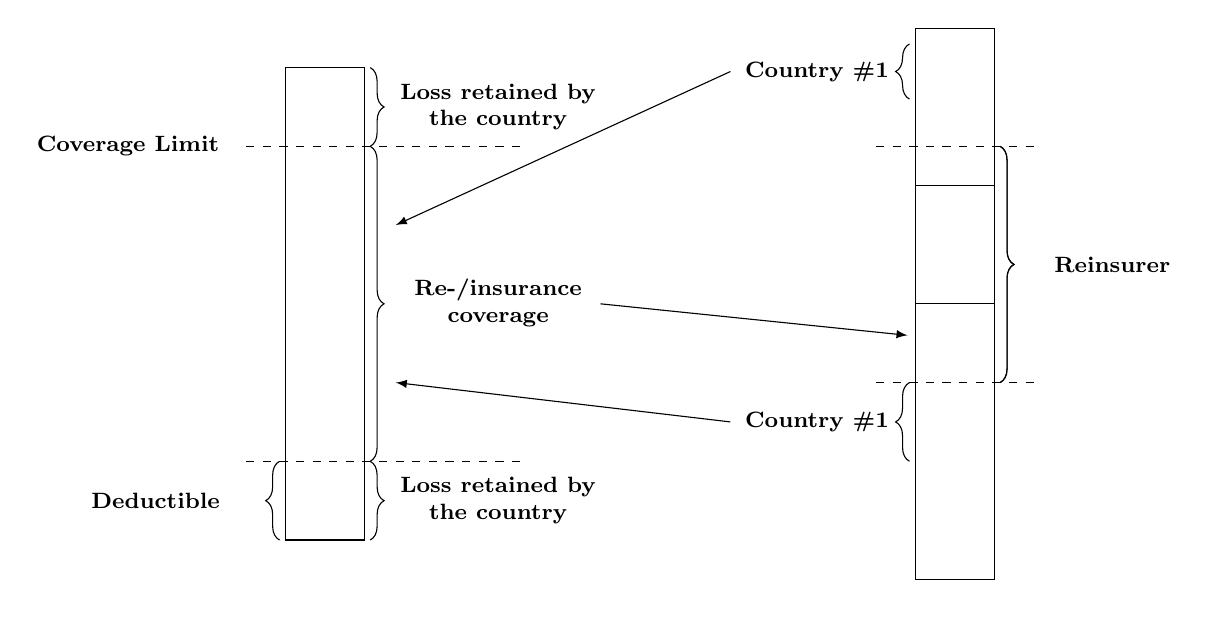
\begin{tikzpicture}[block/.style={rectangle, draw, minimum width=2cm, minimum height=3cm, align=center}]
%%%%%%%%%%%%%%%%%%%
\draw (0,0) rectangle (1,6);
\draw (9,-0.5) rectangle (8,6.5);
\draw[dashed] (-0.5,5) -- (3,5);
\draw[dashed] (-0.5,1) -- (3,1);
\draw[dashed] (7.5,5) -- (9.5,5);
\draw[dashed] (7.5,2) -- (9.5,2);
\draw[black] (8,4.5) -- (9,4.5);
\draw[black] (8,3) -- (9,3);
\draw[->, >=latex] (4,3) -- (7.9,2.6);
\draw[->, >=latex] (5.65,5.95) -- (1.4,4);
\draw[->, >=latex] (5.65,1.5) -- (1.4,2);

%%%%%%%%%%%%%%%%%%%%%
\node[draw=none] at (-2,5) {\bf \footnotesize Coverage Limit};
\node[draw=none] at (-1.65,0.5) {\bf \footnotesize Deductible};
\node[draw=none] at (10.5,3.5) {\bf \footnotesize Reinsurer};
\node[draw=none] at (2.7,0.5) {\bfseries  \footnotesize \begin{tabular}{c} Loss retained by \\  the country \end{tabular}};
\node[draw=none] at (2.7,5.5) {\bfseries \footnotesize \begin{tabular}{c} Loss retained by \\  the country \end{tabular}};
\node[draw=none] at (2.7,3) {\bfseries \footnotesize \begin{tabular}{c} Re-/insurance \\  coverage \end{tabular}};
\node[draw=none, xshift=-1.25cm] at (8,5.95) {\bf \footnotesize Country \#1};
\node[draw=none, xshift=-1.25cm] at (8,1.5) {\bf \footnotesize Country \#1};

%%%%%%%%%%%%%%%%%%%
\draw [decorate,decoration={brace,amplitude=5pt,raise=0.5ex}]
  (0,0) -- (0,1) node[midway,yshift=-3em]{};
\draw [decorate,decoration={brace,amplitude=5pt,mirror,raise=0.5ex}]
(1,0) -- (1,1) node[midway,yshift=-3em]{};
\draw [decorate,decoration={brace,amplitude=5pt,mirror,raise=0.5ex}]
(1,5) -- (1,6) node[midway,yshift=-3em]{};
\draw [decorate,decoration={brace,amplitude=5pt,mirror,raise=0.5ex}]
(1,1) -- (1,5) node[midway,yshift=-3em]{};
\draw [decorate,decoration={brace,amplitude=5pt,mirror,raise=0.5ex}]
(9,2) -- (9,5) node[midway,yshift=-3em]{};
\draw [decorate,decoration={brace,amplitude=5pt,mirror,raise=0.5ex}]
(9,2) -- (9,5) node[midway,yshift=-3em]{};
\draw [decorate,decoration={brace,amplitude=5pt,raise=0.5ex}]
(8,1) -- (8,2) node[midway,yshift=-3em]{};  
\draw [decorate,decoration={brace,amplitude=5pt,raise=0.5ex}]
(8,5.6) -- (8,6.3) node[midway,yshift=-3em]{};  
\end{tikzpicture}
}
\label{fig:CAT}
\end{figure}
An example of decentralized insurance is the catastrophe risk pooling shown in Figure \ref{fig:CAT}, which motivates the formulation of the research question in this paper. The risk pool covers only a portion of each participating country's losses. Any loss below a threshold (say once every five-year event) or the loss exceeding a certain limit (say once every 250-year event) is retained by the country itself. These thresholds are determined by a map of probable maximum loss (loss probability distribution) estimated from historical data. The risk pool is also covered by reinsurance with a deductible and policy limit. The losses below the deductible and above the limit are shared among participating countries in proportion to their mean historical losses. As alluded to earlier, catastrophe risk pooling allows non-member countries to join to boost regional cooperation. The entrance is expected to be approved by all existing member states.  More details can be found in \cite{feng2024unified}. This paper studies precisely this issue of the new entrance. In practice, member states are naturally concerned about their own positions with each expansion of the risk pool. While there are political and other considerations, it is also important to understand the economic consequences of risk pooling. The paper provides a theoretical framework in which members' decision-making is explicitly formulated and analyzed. However, for simplicity, we restrict the attention to the excess-of-loss type of reinsurance contract. The results in this paper can be further extended to more complex decentralized insurance contracts.

We shall formulate the decentralized insurance contract as a combination of a risk-sharing rule $\mathbf{h}$ and a risk-transfer $\mathbf{g}$ such that $g_i(X)= X \wedge d_i+c_i$, where $d_i$ is the deductible of an insurance. The constant $c_i$ is the premium for insurance coverage and ensures the risk-transfer rule, such as the actuarial fairness, {\it i.e.} $\mathbb{E}[g_i(X)]=\mathbb{E}[X]$. This risk-transfer rule is introduced where the risk post-exchange $h_i(\mathbf{X})$ exceeds the risk-bearing capacity of the agent and he chooses to transfer the excessive risk beyond the capacity to a third party such as an insurer. Such a scheme is also referred to as individually covered P2P insurance. If $\mathbf{h}(\mathbf{X})$ is comonotonic and $d_i=h_i(K),$ then such a scheme is equivalent to a group-covered P2P insurance. In a group-covered case, the group of agents buys insurance coverage collectively with a deductible $K$. The insurer underwrites the risk $(S_n-K)_+$ and the risk below the deductible, $S_n\wedge K$, is shared among all agents. This is the reinsurance setting that we shall impose in the sequel. 

\section{Expansion of Risk Pool with Fairness Principle}\label{sec:expansion}

We return to the effects of pool expansion when the side payments (cash transfer inside the group) are given by FP of Definition \ref{def:fairness}. For this, we shall consider the possible expansion of a stable risk pool, under the assumptions of normality and stability \eqref{eq:stabilitycondition}. We first provide the necessary and sufficient conditions for SC. 

\subsection{Strong Consensus and Fairness Principle}
In the view of condition \eqref{eq:stabilitycondition}, we observe that the condition of SC is determined solely by individual and aggregate DTRs. 
\begin{theorem}\label{thm:maintheorem}
The expanded pool reaches SC if and only if DTR of the expanded pool is less than that of the existing pool and that of the candidate, {\it i.e.} 
\begin{align}
\frac{s_{n+1}}{\Delta_{n+1}}\le \min\left\{\frac{s_{n}}{\Delta_{n}},  \frac{\sigma_{n+1}}{\delta_{n+1}}\right\}.\label{ineq:maintheoremcondition}    
\end{align}
\end{theorem}
We note that SC for the existing members occurs when  {$s_{n+1}/\Delta_{n+1}\le s_{n}/\Delta_{n},$ which} determines the {\bf acceptance region by the existing pool}, which has two important features. First, it does not depend on each individual member's mean loss (since they are balanced by the cash transfer). Second, the condition is uniform within the existing pool, {\it i.e.}~ each agent faces the same
condition, which allows us to omit the index ‘$i$’ in the formulation. In other words, under FP, \textit{if one member wants the candidate to join, then everyone else does too}. 
\begin{remark}\label{rmk:either}
  {Thanks to the uniform consensus of existing members under FP, one can show that either the existing pool or the candidate benefits from the pool expansion under the normality assumption.}
\end{remark}
Taking into account the corresponding candidate's condition, that is  {$s_{n+1}/\Delta_{n+1}\le \sigma_{n+1}/\delta_{n+1}$,} we conclude that SC occurs when DTRs of both the expanded pool and the candidate are lower than they are in the status quo. It implies that in order to have SC, the standard deviation of the aggregate risk increases at a slower rate than the tolerance rate of the aggregate risk. This could happen when the variance of the candidate's risk is low and it has a low correlation with the existing group's aggregate risk. Below, we make this statement more precise.  

\subsubsection*{Acceptance Region and Correlation Coefficient}
The following theorem offers upper bounds on the correlation between the aggregate risk of the existing pool and the risk of the candidate.

\begin{corollary}\label{cor:correlation}
The uniform strong-consensus condition   {\eqref{ineq:maintheoremcondition}} is equivalent to
\begin{equation}\label{ineq:rho}
\begin{aligned}
&\rho(S_n,X_{n+1})\leq \frac{(\Delta_{n+1}^2-\Delta_n^2)s_{n}^2-\Delta_n^2\sigma_{n+1}^2}{2\Delta_n^2s_{n}\sigma_{n+1}}\,\,\,\text{ and }\\
&\rho(S_n,X_{n+1})\leq \frac{(\Delta_{n+1}^2-\delta_{n+1}^2)\sigma_{n+1}^2-\delta_{n+1}^2s_{n}^2}{2\delta_{n+1}^2s_n\sigma_{n+1}}.
\end{aligned}
\end{equation}
\end{corollary}
Observe from the first inequality that the upper bound for $\rho$ is increasing in $s_n$ and decreasing in $\sigma_{n+1}$. It means that the acceptable correlation with the candidate's risk is higher when the existing group itself has a high risk or when the candidate has a low risk. The situation is symmetric with the upper bound in the second inequality. The candidate is more willing to enter when bearing high risk and when the existing group has low aggregate risk.  

\subsubsection*{Acceptance Region and Candidate's Variance}

SC can also be expressed in terms of the candidate's variance. In order to focus on the discussion of $\sigma_{n+1}$, we impose the following 
simplified assumption  {$\rho(X_i,X_j)=\rho>0,$ with $i\neq j$ for all $i,j=1,2,...,n+1.$} Pairwise common correlation coefficient is often imposed in problems with multiple agents to help the delivery of economic insights (see among others \cite[Chapter 18]{kpw} for its use and justification in credibility theory).
Define $\Sigma_{n}:=\sum_{i=1}^n\sigma_{i},$ and the condition follows from Theorem \ref{thm:maintheorem}.
\begin{corollary}\label{cor:acceptance}
Under the normality assumption and the common pairwise correlation assumption,   {the condition for SC} reduces to the following condition on the variance of the candidate's risk, $\underline{\sigma} <\sigma_{n+1}< \overline{\sigma},$ where $\overline{\sigma} =-\rho\Sigma_{n}+\sqrt{\left(\rho\Sigma_{n}\right)^2+\left(\frac{\Delta_{n+1}^2}{\Delta_{n}^2}-1\right)s_{n}^2}$ and $\underline{\sigma} =\delta_{n+1}^2\frac{\rho\Sigma_{n}+\sqrt{\left(\rho\Sigma_{n}\right)^2+(\Delta_{n+1}^2-\delta_{n+1}^2)s_{n}^2}}{\Delta_{n+1}^2-\delta_{n+1}^2}.$
\end{corollary}
SC holds when the variance of the candidate's risk falls into a specific interval. In particular, all existing members benefit from the expansion if the candidate's risk is sufficiently low, while only sufficiently high-risk candidates are willing to join the pool (we readily get that $\underline{\sigma}<\overline{\sigma}$). We also directly see that $ \overline{\sigma}$ becomes higher ({\it i.e.}~existing group's acceptance region increases) when the aggregate risk tolerance of the existing group decreases. This means that the more risk-tolerant existing members are, the less they are willing to accept a candidate. Moreover, more risk-tolerant candidates are more likely to be accepted.



% \subsubsection*{Expansion is Desirable by At Least One}
% Thanks to the uniform consensus of existing members under FP, there are only four possible cases regarding the candidate's entrance. Cases: (I) Both existing members and the candidate benefit from the expansion (strong consensus); (II) Existing agents benefit, while the candidate cannot; (III) Existing members do not benefit, while the candidate wants to join; (IV) Neither one wants to expand. One can show that, while Cases (I), (II), and (III) are possible, Case (IV) is not. 
% \begin{theorem} \label{thm:Atleast}
% Under the normality assumption, either the existing pool or the candidate benefits from the pool expansion. 
% \end{theorem}

\subsection{Weak Consensus and Fairness Principle }\label{sec:weakconsensus}
In contrast to SC, WC does not require that each of the existing members is better off with the candidate's entrance. Rather, WC occurs when none of the existing members and the candidate wants to leave the sharing pool due to the candidate's entrance (\textit{i.e.} WC is a weaker condition than SC). As expected, this condition is also determined solely by DTR. 
\begin{theorem}\label{thm:weakconsensus}
Under the normality assumption, the expanded pool reaches WC if and only if DTR of the expanded pool is less than the individual ratio of each of the existing members, that is  
\begin{equation}\label{eq:weakratio}
\frac{s_{n+1}}{\Delta_{n+1}}
\leq \frac{\sigma_{i}}{\delta_i},\quad\forall\, i=1,\cdots, n+1.
\end{equation}
The above condition is equivalent to, for all $i=1,...,n+1,$
\begin{equation}\label{eq:weakcorr}
\rho(S_n,X_{n+1})\leq\frac{\Delta_{n+1}^2\sigma_i^2-\delta_i^2(\sigma_{n+1}^2+s_{n}^2)}{2\delta_i^2s_n\sigma_{n+1}}.
\end{equation}

\end{theorem}

None of the agents leaves the expanded risk pool if and only if the aggregate DTR is lower than that of each individual ratio. Three observations are in order. 
\begin{itemize}
\item {\bf Connection of WC and stability conditions:}
By definition, WC coincides with the stability property of the expanded pool (see also  \eqref{eq:stabilitycondition} and \eqref{eq:weakratio}). Nonetheless, the two conditions are derived from different purposes: The stability refers to the condition under which an existing pool holds together, while WC determines whether a candidate for an expanded pool makes existing members leave the pool. 

\item {\bf Non-uniformity of WC:} In contrast to SC, the condition for WC is not uniform for all agents. Observe that the right-hand side of \eqref{eq:weakratio} is clearly an increasing function of DTR $\sigma_i/\delta_i$. The lowest upper bound for $i=1,\cdots, n+1$ is given by $(\sigma_m/\delta_m):=\min_{1\leq i\leq n+1}(\sigma_i/\delta_i)$. Hence if \eqref{eq:weakratio} holds for $i=m$ then WC is achieved. It is also worthwhile noting that $(\sigma_m/\delta_m)$ decreases with the size of the group. This is consistent with the fact that WC becomes harder to get when the pool gets larger.
\item {\bf Special case where WC holds for all:} An interesting special case is when the common pairwise correlation assumption holds  {such that $
\rho=1$} and all agents are homogeneous. Then, \eqref{eq:weakratio} becomes an equality and hence the expansion of the group with homogeneous agents keeps them indifferent (\textit{i.e.} in a formal sense, WC always holds among homogeneous agents).
\end{itemize}

\subsubsection*{Graphical representations for SC and WC}
  {The left panel in Figure \ref{fig:atleast} illustrates an example for SC,} where axes present the correlation $\rho(S_n,X_{n+1})$ and deviation $\sigma_{n+1}$. The red line and blue line represent the border cases for existing members and the candidate.  For all pairs to the left of the blue line (resp.~right of the red line), the candidate (resp.~the existing pool) benefits from the expansion. Observe that the two lines intersect at the point where $\rho(S_n, X_{n+1})=1$. This means that the intersection, colored yellow, indicates all pairs of SC.  The figure clearly shows that only Cases (I), (II), and (III) are possible, which indicates that at least one party is interested in the expansion. 

  {The right panel in Figure \ref{fig:atleast}} offers an example of WC. If a new member enters the pool, an existing member would exit the pool if the correlation $\rho_{n,n+1}:=\rho(S_n,X_{n+1})$ is higher than the threshold which is the right-hand-side of \eqref{eq:weakcorr}. For example, the first agent's threshold is represented by the dashed green line, where the first agent will leave the pool on the right side of the dashed green line. The lowest threshold for all members is determined by the threshold of the $m$-th member, which is represented by the solid green line. WC holds when $s_{n+1}/\Delta_{n+1}\leq \sigma_m/\delta_m$ from \eqref{eq:weakratio}. In the figure, the intersection of light green-shaded areas is the region where WC occurs, visualized by the dark green-shaded area.
\begin{figure}[t]
\caption{Regions of SC and WC for expansion.}
\centering
\begin{subfigure}[b]{0.45\textwidth}
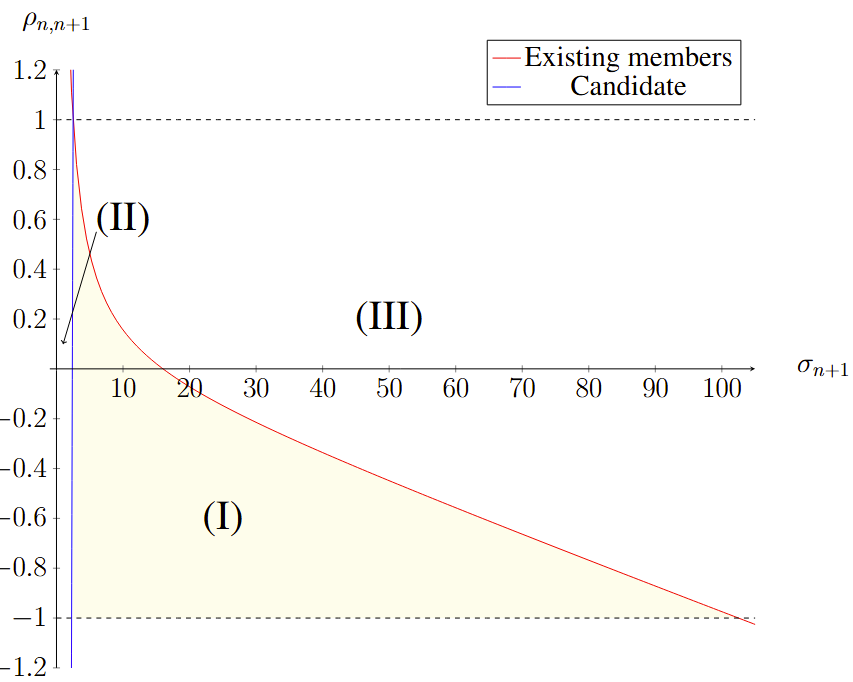
\includegraphics[width=\textwidth]{Figures/SC.png}
\end{subfigure}
\hfill
\begin{subfigure}[b]{0.45\textwidth}
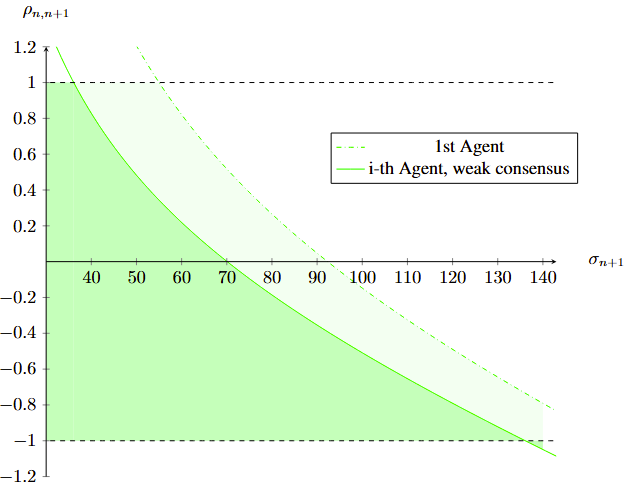
\includegraphics[width=\textwidth]{Figures/WC.png}
\end{subfigure}
\noindent\begin{minipage}{\textwidth}
\raggedright
\NOTE{\\{\it Note}: On the left panel, an example of SC is presented. the vertical axis represents the correlation $\rho_{n,n+1}:=\rho(S_n,X_{n+1})$ and the yellow-shaded area shows where the existing agents and the candidate benefit from the expansion. In this example, $n=20$, $s_n=50$, and the common risk tolerance is set to $\delta=1$. The red line represents the boundary condition for existing members, while the blue line shows that for the candidate. Cases: (I) Both existing members and the candidate benefit from the expansion (SC); (II) Existing agents benefit, while the candidate cannot; (III) Existing members do not benefit, while the candidate wants to join. On the right panel, the vertical axis is the correlation $\rho_{n,n+1}:=\rho(S_n,X_{n+1})$ and the dark green-shaded area is the region of WC. In this example, $n=20$, $s_n=50$, and risk tolerances are fixed by $\delta=1$. It is assumed that $\sigma_1=5$ and $\sigma_m=4$.}
\end{minipage}
\label{fig:atleast}
\end{figure}

\section{Decentralized Insurance Under Fairness Principle}\label{sec:reinsurance}
As alluded to in Section \ref{sec:dein}, participants of risk sharing often want to transfer a portion of their aggregate risk beyond their own financial capacity to a third party. While there are many ways of constructing decentralized insurance pools (c.f. \cite{feng2024unified}), we shall focus on a relatively simple, but widely-used form of {\it excess-of-loss reinsurance}. Any aggregate loss beyond the risk-bearing capacity of the group, $K_n$, is transferred to a reinsurer, {\it i.e.} the portion $(S_n-K_n)_+$ is ceded to a reinsurer. The positive real number $K_n$ shall be referred to as the deductible of the reinsurance. The pool is collectively responsible for losses up to $K_n,$ {\it i.e.} $\overline{S}_n:=S_n \wedge K_n.$ 
As the size of the risk pool, $n$, increases, it is expected that the pool has a larger risk-bearing capacity and hence requires reinsurance of a higher deductible, $K_n$. To make a fair comparison of risk pools with varying sizes, we shall define $\beta$ to measure the extent of reinsurance coverage  {$\beta=(K_i-m_i)/s_i$.} While the size of the risk pool may be different, we shall keep the extent of reinsurance coverage constant for all $i=1,\cdots, n, n+1,\cdots.$
\subsection{Risk Sharing and Actuarial Fairness}
Imposing again the optimal risk-sharing rule under entropic risk measures, we obtain the convex sharing of the aggregate risk covered by the pool, {\it i.e.} the allocated risk for the $i$-th member under reinsurance is changed to $\overline{Y}_{n,i}=\lambda_{n,i} \overline{S}_n+c_i$ for $i=1,\cdots, n,$ where $c_i$ is the cash payment that aims to ensure fairness for all members (and the reinsurer). As discussed in Section \ref{sec:classic}, this result can also be obtained from the general representation of a decentralized insurance scheme $\overline{\mathbf{Y}}=\mathbf{g}\circ \mathbf{h}(\mathbf{X})$. In the risk-sharing step, we set $h_i(\mathbf{X})=\lambda_{n,i} S_n$. In the risk-transfer step, the risk retention is given by $g_i(Y)=Y\wedge d_i+c_i$ where the agent's risk-bearing limit is determined by $d_i=\lambda_{n,i}K_n$  for $i=1,\cdots, n.$ Then each agent's retained risk can be represented by $\overline{Y}_{n,i}= g_i\circ h_i(\mathbf{X})=\lambda_{n,i} \overline{S}_n+c_i.$ The decentralized insurance scheme is said to be actuarially fair if $c_i=\mathbb{E}[X_i]-\mathbb{E} [\lambda_{n,i}\overline{S}_n].$
If the reinsurance premium paid by the group to the reinsurer is also determined by actuarial fairness, then $c^{(n)}:=\EE[(S_n-K)_+].$ It is clear that all members' cash payments add up to that to the reinsurer, {\it i.e.} $c^{(n)}=\sum^n_{i=1} c_i.$

Under actuarial fairness, we shall point out that a critical quantity for comparing ``the welfare" of members (as determined by the entropic risk measure) is given by
\begin{equation}\label{eq:EE_i}
\begin{aligned}
\mathcal{E}_i[X]&=\log  \mathbb{E}\left[\exp\left\{\frac1{\delta_i}(X-\mathbb{E}[X])\right\}\right]\\
&=\frac{1}{\delta_i}\left(\rho_i(X_i)-\EE[X]\right).
\end{aligned}
\end{equation}
If $X$ is normally distributed with variance $\sigma^2$, it immediately follows that  {$\mathcal{E}_i[X]=l\left(\sigma/\delta_i\right),$ where $l(x):=x^2/2.$} Hence, under the normality assumption, $S_n$ is also normally distributed and hence  {$\mathcal{E}_i[\lambda_i S_n]=l\left(s_n/\Delta_n\right).$}
Observe that $\overline{S}_n$ has a truncated normal distribution, whose moment generating function is also well-known. In particular, we have that  {$\mathcal{E}_i[\lambda_{n,i} \overline{S}_n]=l\left(s_n/\Delta_n;\beta \right),$} where   {$l(x;\beta):=\log\left(e^{\frac{x^2}{2}}\Phi\left(\beta-x\right)+e^{\beta x}(1-\Phi(\beta))\right)+ x\left(\phi(\beta)-\beta(1-\Phi(\beta))\right)$ such that} $\phi(\cdot)$ and $\Phi(\cdot)$ are the normal density and cumulative distribution functions, respectively. Note that 
$\lim_{\beta\rightarrow \infty}l(x;\beta)=l(x)$, which is the case without reinsurance. 

\subsection{Effect of Reinsurance}\label{sec:Dec_eff_Rein}
This setting guarantees that the reinsurance benefits all the existing members of the pool.  {Specifically, under the normality assumption and the actuarial fairness, for every level of $\beta$, the reinsurance makes agent $i$  better off if and only if $\mathcal{E}_i[\lambda_{n,i} S_n]\ge \mathcal{E}_i[\lambda_{n,i} \overline{S}_n],$ where the map $\mathcal{E}_i$ is defined in \eqref{eq:EE_i}, for each $i=1,\dots,n$.} We readily get that  {this condition} is uniform for all agents (just like the condition for SC \eqref{ineq:maintheoremcondition}). Indeed,  {it} is equivalent to $\frac{1}{2}\left(s_n/\Delta_n\right)^2\geq l\left(s_n/\Delta_n;\beta\right),$ for any given $\beta$, which is proved in the next theorem.
\begin{theorem}\label{thm:fair_reinsualwaysbetter}
Under the normality assumption and the actuarial fairness, the reinsurance always makes each existing member better off.
\end{theorem}
  {Theorem \ref{thm:fair_reinsualwaysbetter} implies the following remark.}
\begin{remark}
  {Since reinsurance makes each member better off, it is also beneficial in welfare sense. In fact, each member is willing to pay an extra premium for reinsurance, on top of the actuarially fair premium (see Appendix E.1 % \ref{app:extra_prem}
for details).}
\end{remark}

\subsection{Stability and Weak Consensus with Reinsurance}
Intuitively, the reinsurance should enhance the existing pool's stability because all agents in the pool benefit from the reinsurance. Indeed, let $x=s_n/\Delta_n$ be DTR of the group and $z_i=\sigma_i/\delta_i$ be that of $i$-th agent. Consider stability regions for the $i$-th agent with and without reinsurance $O_i:=\{(x,z): x,z_i>0,\, x^2/2\leq z_i^2/2\}$ (corresponding to \eqref{eq:stabilitycondition}) and $\overline{O}_i=\{(x,z): x,\beta,z_i>0,\, l(x;\beta)\leq z_i^2/2\},$ respectively. By Theorem \ref{thm:fair_reinsualwaysbetter}, $x^2/2\leq z_i^2/2 $ implies $l(x;\beta)\leq z_i^2/2.$ Therefore, the region $\overline{O}_i$ is always wider than the region $O_i$ for each $i$, {\it i.e.}, the region for stability becomes wider with the reinsurance.

This argument also holds for WC, when a candidate enters the pool. Recall that WC requires the comparison of an individual's stand-alone risk and the risk after the risk sharing in the expanded pool. Intuitively, the reinsurance benefits each member and enhances WC.

\begin{theorem}\label{thm:fair_rein_weakstab}
Under the normality assumption and the actuarial fairness, regions for stability and WC become wider with the reinsurance.
\end{theorem}

\subsection{Strong Consensus with Reinsurance}\label{sec:existingreinsu}
It is known from Theorem \ref{thm:maintheorem} that SC without reinsurance is determined solely by DTRs. This is also the case under reinsurance, although reinsurance reduces the risk for each agent (and hence alters   {the condition for SC}).
\begin{theorem}\label{thm:rein_strong}
Under the normality assumption and FP, the expanded pool reaches SC if and only if the condition holds 
\begin{equation}\label{eq:rein_strong}
l\left(\frac{s_{n+1}}{\Delta_{n+1}},\beta\right)\leq \min\left\{l\left(\frac{s_{n}}{\Delta_{n}},\beta\right),\frac{1}{2}\left(\frac{\sigma_{n+1}}{\delta_{n+1}}\right)^2\right\},
\end{equation}
where the function   {$l(x;\beta)$ is defined as above.}
\end{theorem}
The first required inequality $l(s_{n+1}/\Delta_{n+1},\beta)\leq l(s_{n}/\Delta_{n},\beta)$ is the condition for the existing members, while the second inequality $l(s_{n+1}/\Delta_{n+1},\beta)\leq (\sigma_{n+1}/\delta_{n+1})^2/2$ refers to the candidate's willingness to join the pool. Condition \eqref{eq:rein_strong} reflects the way that the much simpler condition \eqref{ineq:maintheoremcondition} is altered due to the presence of reinsurance coverage. In other words, the extended aggregate DTR is compared only through function $l$ with the old one, while its comparison with the candidate's ratio is through different functions. Note that condition \eqref{eq:rein_strong} converges to \eqref{ineq:maintheoremcondition} when $\beta\to\infty$, {\it i.e.} when reinsurance vanishes. 

\subsubsection*{Effect of Reinsurance on Acceptance Region}\label{sec:changeinaccept}
Using similar arguments to those for Theorem \ref{thm:fair_reinsualwaysbetter} (willingness of existing members to accept a candidate under WC), one can show that reinsurance would increase the willingness of the candidate to join the pool.   {On the other hand, due to the monotonicity of the function $l$ under certain condition on $\beta,$ \eqref{eq:rein_strong} and \eqref{ineq:maintheoremcondition} produce the same acceptance region for SC.}
\begin{theorem}\label{thm:acceptchange_candidate}
Under the normality and the constant coverage ratio assumption, the candidate's acceptance region with reinsurance is wider than or equal to his acceptance region without reinsurance   {for any level of $\beta$. Moreover, if $s_{n+1}/\Delta_{n+1}, s_{n}/\Delta_{n}>  {\beta+1/\beta}$,} then the acceptance region of existing members is the same with and without reinsurance.
\end{theorem}
% The comparison of conditions is illustrated in Figure \ref{fig:compare}. Let $x=s_{n}/\Delta_{n}$, $y=s_{n+1}/\Delta_{n+1}$, and $z=\sigma_{n+1}/\delta_{n+1}.$ The orange-shaded area represents the region where the existing members and the candidate agree to the expansion in the absence of reinsurance, while the blue-shaded area shows that in the presence of reinsurance. As Theorem \ref{thm:acceptexisting} suggests, existing members' acceptance regions with and without reinsurance overlap in Figure \ref{fig:compare_exist}. Figure \ref{fig:compare_candidate} shows the change of acceptance region for the candidate. The candidate is more willing to join the risk pool since the blue-shaded area extends beyond the orange-shaded area. 
% \begin{figure}[t]
% \centering
% \caption{Comparison of acceptance region with and without reinsurance under strong consensus when $\beta=1.96.$ }
% \resizebox{0.7\textwidth}{!}{%
% \begin{subfigure}[b]{0.30\textwidth}
% \centering
% \includegraphics[width=\textwidth]{Figures/20230516_Tuesdays_existing_compare.jpg}
% \subcaption{}
% \label{fig:compare_exist}
% \end{subfigure}
% \hspace{0.1\textwidth}
% \begin{subfigure}[b]{0.30\textwidth}
% \centering
% \includegraphics[width=\textwidth]{Figures/20230516_Tuesdays_candidate_compare.jpg}
% \subcaption{}
% \label{fig:compare_candidate}
% \end{subfigure}
% }
% % \NOTE{\\ {\it Note}: As expected, the acceptance region is the same in both cases for the existing members. It is wider than or equal to the one without reinsurance for the candidate.}
% \label{fig:compare}
% \end{figure}
In summary, under FP, individual and aggregate DTRs determine SC and WC. In particular, the pool reaches SC if the existing pool and candidate's ratio are both higher than the ratio of the extended pool. This means that the existing pool does not accept candidates with sufficiently risky positions. On the other hand, WC holds when the expanded pool's ratio stays lower than the individual DTR of each member. While reinsurance makes WC more likely, it positively affects only the candidate's decision to enter the pool.

\section{Expansion of Risk Pool Under Equilibrium Priciple}\label{sec:equilibrium}

In the previous analysis, the pricing of cash transfers is always based on actuarial fairness, which is a pricing rule that takes into account only the expectation under a common probability measure. There are two main advantages to this pricing rule: its simplicity and the uniformity of SC when the pool's expansion is considered. However, imposing a pricing rule that considers only the risks' expectations comes with some disadvantages. It does not guarantee the stability (or the incentive to participate in) of the pool. Recall from Section \ref{subsec:stability} that, under the normality assumption, the pool is stable if and only if \eqref{eq:stabilitycondition} holds. Members stay in the risk pool only if their individual DTRs are sufficiently high. A direct consequence is that agents with risks of low variance and low-risk aversion have less incentive to participate in the risk pool, or equivalently, only members with risks of high variance and high-risk aversion find it attractive to trade risks. In fact, the linear pricing rule does not penalize the risks with high variance and hence existing members are less willing to accept candidates with high risk. Such a feature reduces sharing efficiency, in the sense that agents with higher risk will not be accepted in a pool with lower risk agents, although a mutually beneficial sharing among agents with different levels or risks is possible.

   {In order to deal with the aforementioned disadvantages we need to impose a risk-adjusted pricing rule for the side payments, that penalizes the agents with higher risk and still be consistent with the competitive structure. For this we propose a pricing rule which is based on the equilibrium principle (EP) upon the transaction of risks. More precisely, since under the entropic risk measure the optimal sharing is linear, we may consider each agent's risk as tradable asset and the risk allocation could be determined by a market-clearing condition, {\it i.e.}~when optimal demands sum up to zero. In fact, as it is shown in \cite{anthropelos2010agent} (see also \cite{anthropelos2010agent2} where the aforementioned equilibrium principle idea is developed for general convex risk measures) the induced equilibrium is consistent with Pareto optimal risk sharing, whereas EP is still an expected value but under a different (than the initial) endogenously derived probability measure. Below, we describe equilibrium arguments in a risk pool.}


Let $\tb{X}=(X_1,X_2,...,X_n)$ be the vector of all agents' risks that are now considered as ``assets'' whose prices are given by a real-valued vector $\tb{p}=(p_1,p_2,...,p_n)\in\mathbb{R}^n$. The demand function of each agent $i$ at a given price vector $\tb{p}$ is given as the position on each asset that minimizes its risk, that is
\begin{equation}\label{eq:individual_demand}
\begin{aligned}
\mathbf{z}_{i}^*(\tb{p}):&=\underset{\mathbf{z}\in\mathbb{R}^n }{\arg \min }\,
\rho_i(X_i+\tb{z}^\top\tb{X}  {-\tb{z}^\top\tb{p})}
% &=\underset{\mathbf{z}\in\mathbb{R}^n }{\arg \min }
% \left\{\rho_i(X_i+\tb{z}^\top\tb{X})+\tb{z}^\top\tb{p}\right\},  
\end{aligned} 
\end{equation}
for each $i=1,2,\dots,n,$  {where $\tb{z}^\top\tb{p}$ denotes the cash received by the agent in order to undertake risk $\tb{z}^\top\tb{X}$. Then the market clearing condition is $\sum_{i=1}^n\tb{z}^*_i(\tb{p}^*)=0$.} Based on the arguments of \cite[Proposition 2.1]{anthropelos2010agent}, we may rewrite the above equilibrium setting in an aggregate level (using the notation of the previous sections) in the following way: The equilibrium market-clearing optimal sharing is determined by the solution of the minimization problem  
\begin{equation}\label{demand}
\begin{aligned}
&\underset{\mathbf{A}_{n\times n}}{\arg \min } \sum_{i=1}^n
\rho_i(Y_i), \\
&\quad \mathbf{Y}:=(Y_1,Y_2,\dots,Y_n)=\mathbf{A}\mathbf{X}  {-\mathbf{A}\mathbf{p}+\mathbf{p},}
\end{aligned}
\end{equation}
where the market-clearing condition takes the form $\mathbf{e}^\top \mathbf{A}=\mathbf{e}^\top$ with $\tb{e}:=(1,1,\dots,1)\in\mathbb{R}^n$. In the above formulation, rows of matrix $\mathbf{A}$ represent agents' allocations, that is the $i$-th row is the allocation of the agent $i$'s risk. Connecting the above with the demand function \eqref{eq:individual_demand}, we have at equilibrium that $\tb{z}_i^*(\tb{p}^*)=\mathbf{a}_{i}^*-\tb{e}_{i},$ where $\tb{e}_{i}^\top=(0,\cdots,1,\cdots,0)$ such that $1$ is at the $i$-th element. Note that even without the normality assumption, problem \eqref{demand} admits a unique solution if simple regularity conditions on $X_i$'s hold. 

  {Since the problem \eqref{demand} is strictly convex, the unique equilibrium can be derived, under the normality assumption, i.e. $\mathbf{X}\sim\text{Normal}(\boldsymbol{\mu}, \boldsymbol{\Sigma})$}, from the following equation
\begin{equation}\label{eq:equilibrium measure}
\mathbf{\mathbb{E}}\left[\frac{e^{(\mathbf{a}^*_{i}) ^\top\tb{X}/\delta_i}}{\mathbb{E}[e^{(\mathbf{a}^*_{i}) ^\top\tb{X}/\delta_i}]}\mathbf{X}\right]=\mathbf{p}^*
\end{equation}
where $(\mathbf{a}_{i}^*)^\top$ is the $i$-th row of the equilibrium allocation $\mathbf{A}^*$. In fact, the optimal allocation $a_i^*$ coincides with the Pareto allocation (see again \cite{anthropelos2010agent}) such that $\mathbf{a}_{i}^*=(\lambda_{n,i},\lambda_{n,i},\lambda_{n,i},\cdots,\lambda_{n,i})^\top=\lambda_{n,i}\tb{e}$ for all $i=1,2,...,n.$ The cash transfer is 
\[ {-(\tb{z}^*)^\top\tb{p}^* =\mathbf{p}^*-\mathbf{A}^* \tb{p}^*}=\left(\mathbf{I}-\mathbf{A}^*\right)\left(\frac{1}{\Delta_n}\mathbf{\Sigma e}+\boldsymbol{\mu}\right).
\]
% \textcolor{blue}{The problem \eqref{demand} is strictly convex and its FOCs are, for all $i=1,2,...,n,$
% \[
% \frac{\partial \rho_i(Y_i)}{\partial \mathbf{a}_i^*}=
% \begin{pmatrix}
% \frac{\partial\rho_i(Y_i)}{\partial a_{i1}^*}&
% \frac{\partial\rho_i(Y_i)}{\partial a_{i2}^*}&
% \cdots&
% \frac{\partial\rho_i(Y_i)}{\partial a_{in}^*}
% \end{pmatrix}^\top=0
% \]
% where $(\mathbf{a}_{i}^*)^\top$ is the $i$-th row of the equilibrium allocation $\mathbf{A}^*$. This implies that the 
% for each $i$, the equilibrium price $\mathbf{p}^*$ satisfies the following condition
% \begin{equation}\label{eq:equilibrium measure}
% \mathbf{\mathbb{E}}\left[\frac{e^{(\mathbf{a}^*_{i}) ^\top\tb{X}/\delta_i}}{\mathbb{E}[e^{(\mathbf{a}^*_{i}) ^\top\tb{X}/\delta_i}]}\mathbf{X}\right]=  {-\mathbf{p}^*}
% \end{equation}
% This is an implicit form of the demand. From the above condition, we obtain the unique equilibrium (under the normality assumption), and in fact, the optimal allocation $a_i^*$ coincides with the Pareto allocation (see again \cite{anthropelos2010agent}). More precisely, we obtain that $\mathbf{a}_{i}^*=(\lambda_{n,i},\lambda_{n,i},\lambda_{n,i},\cdots,\lambda_{n,i})^\top=\lambda_{n,i}\tb{e}$ for all $i=1,2,...,n,$ where we recall that $\lambda_{i}=\delta_i/\Delta_{n}$. Then, the equilibrium price is
% \begin{equation}\label{eq:price}
% \left.\frac{\partial \rho_i(Y_i)}{\partial \mathbf{a}_i^*}\right|_{\mathbf{a}_i^*=\lambda_{n,i}\mathbf{e}}=\mathbf{\mathbb{E}}\left[\frac{e^{S_n/\Delta_n}}{\mathbb{E}[e^{S_n/\Delta_n}]}\mathbf{X}\right]=  {-\mathbf{p}^*}
% \end{equation}
% Imposing the normality assumption, we obtain that the equilibrium price vector is given by
% \[
%   {-\tb{p}^*}=\mathbb{E}\left[\frac{e^{S_n/\Delta_n}}{\mathbb{E}[e^{S_n/\Delta_n}]}\mathbf{X}\right]=\frac{1}{\Delta_n}\mathbf{\Sigma e}+\boldsymbol{\mu}.
% \]
% Therefore, the cash transfer is
% \[
%   {\mathbf{A}^* \tb{p}^*-\mathbf{p}^*}=\left(\mathbf{I}-\mathbf{A}^*\right)\left(\frac{1}{\Delta_n}\mathbf{\Sigma e}+\boldsymbol{\mu}\right).
% \]
% }
As expected,   {the premium under EP} is different than the one induced by FP. While FP charges the fee equal to the expectation of the risk, EP charges based on both the expectation and the variance of the risk  {\textit{i.e.} a risk-adjusted pricing rule}. Note that the pricing remains an expectation of risks but under a different measure, since we may define measure $\QQ$, through a Radon-Nikodym derivative $d\QQ/d\PP=e^{S_n/\Delta_n}/\EE[e^{S_n/\Delta_n}]$ and the equilibrium pricing   {\eqref{eq:equilibrium measure} becomes 
$\tb{p}^*=\EE_{\QQ}[\tb{X}]$.}

As before under FP, agent $i$ receives the risk $\lambda_{n,i}S_n$ under EP. While her cash transfer is given by  {$\pi_{n,i}=\mu_i-\lambda_{n,i}m_n$} under FP, it changes to  {$\hat{\pi}_{n,i}=\mu_i-\lambda_{n,i}m_n+(1/\Delta_n)\Cov(X_i-\lambda_{n,i}S_n,S_n)$} under EP. In other words, in comparison with that under FP, the agent pays an extra (possibly negative) amount under EP  {$\hat{\pi}_{n,i}-\pi_{n,i}=\Cov\left(X_i,S_n/\Delta_n\right)-\delta_is_n^2/\Delta^2_n.$} Hence, under EP, agents with higher risk ({\it i.e.}~high variance) and risk aversion pay more than under FP.

\subsection{Stability and Weak Consensus under Equilibrium Principle}\label{sec:newpricing_stability}  
One of the main advantages of EP is that the stability condition always holds   {by construction.} Indeed, since each agent submits a demand of each risk, a possible optimal demand is $\tb{e}_i$,   {meaning} that the agent $i$ stays with his initial risk exposure and does not participate in the sharing. In other words, participating in the risk pool cannot be worse than staying outside of it. We readily get that the stability condition is equivalent to 
\begin{align}
\rho_{i}(X_i)-\rho_{i}\left(Y_i\right)
&=\frac{1}{2\delta_i}\Var((\mathbf{a}_{i}^*-\mathbf{e}_{i})^\top\mathbf{X})\geq 0,\label{ineq:equi_stab_weak}
\end{align}
which means that agent $i$ receives strict risk reduction by participating in the risk pool if and only if $\lambda_{n,i}S_n-X_i$ is not constant. The latter is a special case where agents' risks are linearly independent.

As expected, this desired property holds for WC too. As already mentioned, the difference between the stability condition and WC is that the former considers only the pool's existing members, while the latter considers the candidate too. Hence, under EP, WC for the pool expansion always holds and in fact, for each agent, the risk reduction that stems from participation in the pool is strict if and only if $\lambda_{n+1,i}S_{n+1}-X_i$ is not a constant. 
We state the above observations in   {Theorem \ref{thm:eq_weak_stability}}. Note that due to Theorem \ref{thm:eq_weak_stability}, Remark \ref{rmk:either} also holds under EP, since at least a candidate is always willing to enter the group. 
\begin{theorem}\label{thm:eq_weak_stability}
Under EP, both stability and WC always hold. 
\end{theorem}

\subsection{Strong Consensus under Equilibrium Principle}
While both stability and WC are guaranteed under EP, SC becomes more tricky than that under FP. Since the riskiness of each agent's position is penalized under EP, a candidate with higher risk increases the total risk but also pays a high premium to existing members. This possibly makes the entrance of a risky candidate preferable for existing members, a feature that comes in sharp contrast to FP. Another interesting feature is that the condition of SC depends only on existing members, since under EP a candidate is always better off by entering the risk pool (similarly to WC). 

Based on the notation from previous sections, we denote by $\mathbf{X}^{(n)}$ the vector of $n$ agents' risks (the existing members) and by $(\mathbf{A}^{(n)*}, \mathbf{p}^{(n)*})$ the corresponding equilibrium allocation and prices (recall that $(\mathbf{a}_{i}^{(n)*})^\top$ stands for the $i$-th row of $\mathbf{A}^{(n)*}$). Simple calculations lead to the following result (see also \cite[Corollary 2.6]{anthropelos2017}).
\begin{theorem}\label{thm:newpricing_mainthm_withoutsamecorr}
Under EP, the risk measure of a candidate never increases by entering a risk pool. With the normality assumption, the risk measure of existing member $i$ decreases (or stays indifferent) by the candidate's entrance if and only if   {$\Var((\mathbf{a}_{i}^{(n)*}-\mathbf{e}_{i}^{(n)})^\top\mathbf{X}^{(n)})\leq\Var((\mathbf{a}_{i}^{(n+1)*}-\mathbf{e}_{i}^{(n+1)})^\top\mathbf{X}^{(n+1)*}),$} equivalently 
\begin{equation}\label{eq:entrance with new}
\Var(\lambda_{n,i}S_n-X_i)\leq \Var(\lambda_{n+1,i}S_{n+1}-X_i).
\end{equation}
\end{theorem}
Two comments are in order regarding condition \eqref{eq:entrance with new}. First, unlike FP, the equilibrium does not imply the uniformity of SC. Second, \eqref{eq:entrance with new} indicates two opposite effects of the candidate's variance on each existing member's risk measure after the expansion. On one hand, the expansion with a high risk improves each existing member's cash inflow. On the other hand, each of them has to bear a higher risk than otherwise permitted under FP.  

More precisely, \eqref{eq:entrance with new} can be written as an inequality of a second-order polynomial with respect to $\sigma_{n+1}$. In order to focus on variances, we impose for now the common pairwise correlation assumption. Upon defining $\boldsymbol{\delta}=(\delta_i)_{i=1,...,n}$, $\boldsymbol{\sigma}=(\sigma_i)_{i=1,...,n}$, and $\Sigma^{(n)}_{-i}:=\sum_{j\neq i}^{n}\sigma_j$, we find the equivalency of \eqref{eq:entrance with new} to the inequality   {$f_i(\sigma_{n+1}|\,\rho,\boldsymbol{\sigma},\boldsymbol{\delta})\geq 0,$} where, for each 
$i=1,2,...,n$, $f_i(\cdot|\,\rho,\boldsymbol{\sigma},\boldsymbol{\delta})$ is a second-order polynomial defined on the positive real line given by
\begin{equation}
\begin{aligned}
&f_i(x|\,\rho,\boldsymbol{\sigma},\boldsymbol{\delta}):=x^2+2\rho\left(\Sigma^{(n)}_{-i}-\sigma_i\frac{1-\lambda_{n+1,i}}{\lambda_{n+1,i}}\right)x\\
&+2\left(\frac{\lambda_{n,i}-\lambda_{n+1,i}}{\lambda_{n+1,i}^2}\right)\left(\sigma_i^2+\rho\sigma_i\Sigma^{(n)}_{-i}\right)-\left( \frac{\lambda_{n,i}^2}{\lambda_{n+1,i}^2}- 1\right)s_n^2.
\end{aligned}
\label{eq:withsamecor}
\end{equation}
  {Simplifying, $f_i(x|\,\rho,\boldsymbol{\sigma},\boldsymbol{\delta})=(x-b_i)^2-c_i$ such that $b_i:=\rho\left(\sigma_i(1/\lambda_{n+1,i}-1)-\Sigma^{(n)}_{-i}\right)$ and $c_i=-f_i(b_i|\,\rho,\boldsymbol{\sigma},\boldsymbol{\delta}).$} Note that $b_i$ is the deviation of the candidate's risk at which agent $i$ receives the lowest benefit from the candidate's entrance. Clearly, there are three possible cases of $\sigma_{n+1}$ that could yield positive effect of the candidate's entrance to agent $i$'s welfare: (I) only for sufficiently large $\sigma_{n+1}$ (when $b_i^2\leq c_i $); (II) for sufficiently low and sufficiently large $\sigma_{n+1}$ (when $0<b_i$ and $0<c_i\leq b_i^2 $); and (III) for all values of $\sigma_{n+1}$ (otherwise).

\subsubsection*{Effect of Candidate's Entrance on Agents}

As before, we focus on the perspective of agent $i$. The situation is summarized in Table \ref{tab:table1}. Case (I) is straightforward because the agent can be well compensated by the cash transfer from a candidate with sufficiently large risk. In this case, the existing members partially play the role of reinsurer of the candidate's risk, in the sense that he pays a risk-adjusted premium to share his high risk with the existing members.

The other two cases are possible depending on the relative riskiness and risk tolerance of existing members. It is rather easy to find (see also the proof of Theorem \ref{thm:cases for agent i}) that $b_i^2\leq c_i$ holds if $\sigma_i$ is sufficiently low, meaning that an agent with low risk is willing to accept only highly risky candidates (due to the relatively large premium they have to pay under equilibrium principle). The following theorem is qualitatively equivalent to Table \ref{tab:table1} (the exact calculations and thresholds are given in the proof developed in the Appendix). 

\begin{table}[t]
\caption{Regions for $b_i$ and $c_i$ where agent $i$ benefits from the expansion depending on the variance $\sigma_{n+1}$.}
\small
\begin{adjustbox}{center}
\begin{tabular}{|c||c|c|}
\hline
Regions & $b_i\leq0$ & $b_i> 0$\\ \hline\hline
$c_i<0$& Always & Always\\ \hline
$0\leq c_i<b_i^2 $& Always& For sufficiently low and large $\sigma_{n+1}$            \\ \hline 
$b_i^2\leq c_i $ & For sufficiently large $\sigma_{n+1}$ & For sufficiently large $\sigma_{n+1}$ \\ \hline
\end{tabular}
\end{adjustbox}
\NOTE{\\\\ {\it Note}: In the table, sufficiently low means $\sigma_{n+1}<b_i-\sqrt{c_i}$ and sufficiently large means $\sigma_{n+1}>b_i+\sqrt{c_i}$.}
\label{tab:table1}
\end{table}

\begin{theorem}\label{thm:cases for agent i}
Under the normality assumption and the common pairwise correlation assumption,
\begin{itemize}
\item[i.] When $\sigma_i$ is sufficiently low,  agent $i$'s risk measure only decreases with the entrance of a candidate with sufficiently large $\sigma_{n+1}$.

\item[ii.] When $\sigma_i$ is sufficiently large and  $\rho$ is sufficiently high, 
agent $i$'s risk measure decreases with a candidate with sufficiently large and sufficiently low $\sigma_{n+1}$.

\item[iii.] When $\sigma_i$ is sufficiently large and $\rho$ is sufficiently low, agent $i$'s risk measure always decreases with a new member.
\end{itemize}
\end{theorem}

The intuition of the above outcome is clear and reasonable: The first item implies that an existing agent with low risk always prefers a candidate with high risk because of the large side payment. As mentioned above, this situation looks like the relation between an agent (the candidate) who wants to insure some of his risk and an insurer who covers it with a risk-adjusted premium. This situation always holds if the candidate's risk is sufficiently larger than those of the existing member. On the other hand, when an existing member has a relatively high risk and the benefit from diversification is low (high-risk correlation) there is a factor with the opposite direction: an existing member may want to partially insure his risk (and the candidate risk with low becomes the insurer). Combining the first two cases, we may have an ideal situation when the benefit from diversification is high enough (\textit{i.e.} the correlation of risks is low) where the candidate's entrance is beneficial no matter who plays the role of the insurer.

\subsubsection*{Conditions for Strong Consensus}

  {For SC}, we obtain from Theorem \ref{thm:cases for agent i} that a high correlation of risks reduces the region of existing members' acceptance of the candidate since they become less likely to accept additional risk into the pool. This is highlighted when agents have the same risk tolerance.
\begin{corollary}\label{cor:equistrong_prop4}
Consider the case where $\delta_i=\delta$, for all $i=1,2,...,n+1$, under the normality assumption and the common pairwise correlation assumption. When $\rho$ is sufficiently close to one, then none of the existing members always accepts the candidate.
\end{corollary}  
  {The common risk tolerance assumption} is necessary for the above statement   {(a counter-example is presented in Appendix F.1% \ref{app:eg:counter_cor3}
).} Following the discussion above, we impose the normality and the common pairwise correlation assumptions, and return our attention to SC. For each $i=1,...,n$, define the set $\mathcal{A}_i \subseteq \mathbb{R}_+ $ to consist of the values of $\sigma_{n+1}$ for which agent $i$ is willing to accept the candidate. Hence, SC occurs when 
\begin{equation}\label{eq:strong_consensus_equilibrium}
\sigma_{n+1}\in \mathcal{A}:=\bigcap_{i=1}^n\mathcal{A}_i.    
\end{equation}
Theorem \ref{thm:cases for agent i} yields further results regarding SC. Firstly, there is in general no uniformity in contrast to FP. However, condition \eqref{eq:withsamecor} does not depend on risk expectations, which are balanced again by the cash transfer. We also verify that $\mathcal{A}$ is never empty, since existing members benefit from the entrance of a candidate with sufficiently large risk. While SC condition is not uniform in general, we are able to identify which existing member determines the boundaries of $\mathcal{A}$. This stems from the fact that low-risk members prefer a candidate with sufficiently high risk and veto an acceptance of a low-risk candidate, while high-risk members reject a high-risk candidate. The discussion   {is} summarized as follows.
\begin{theorem}\label{thm:strong consensus equilibrium 1}
Under the normality assumption and the common pairwise correlation assumption, the following statements are true.
\begin{itemize}
\item [i.] SC always occurs for sufficiently high $\sigma_{n+1}$.
\item[ii.] When $\sigma_{n+1}$ is sufficiently low, SC is determined by the existing member with low DTR and high risk tolerance.
\item[iii.] When $\sigma_{n+1}$ is sufficiently high, SC is determined by the existing member with high DTR.
\end{itemize}
\end{theorem}
Due to the lack of a uniform condition for SC, the heterogeneity of existing members is an important factor. On the other hand, homogeneity simplifies not only the related formulas but also the intuition of condition for SC. Motivated by the second item of Theorem \ref{thm:strong consensus equilibrium 1}, we examine the case of existing members with the same risk (with and without different risk tolerances). Surprisingly, when existing members have risks with equal variances and equal risk tolerances, SC always holds.

\begin{theorem}\label{thm:common sigma}
Consider the normality assumption and the common positive pairwise correlation assumption and further assume that $\sigma_i=\sigma$, for each $i=1,2,...,n$. When existing members have common risk tolerance, SC always holds for all $(\sigma_{n+1},\delta_{n+1})\in\mathbb{R}^2_+$. This statement does not hold when risk tolerance is different for at least a pair of existing members. In fact, under different risk tolerances, the set $\mathcal{A}$ may be a union of three non-overlapping intervals.
\end{theorem}

When $\mathcal{A}$ is a union of non-overlapping intervals, SC occurs for low, high but also medium values of the candidate's risk. This could also occur when the existing members' heterogeneity stems from different risks (while having the same risk tolerance). 
\begin{theorem}\label{thm:common tolerance}
Consider the normality assumption and the common pairwise correlation assumption. For heterogeneous agents, having $\mathcal{A}$ being a union of three non-overlapping intervals is possible even when $\delta_i=\delta$, for all $i=1,...,n+1$.
\end{theorem}

\subsubsection*{Comparison of Pricing Principles}
It should be clear from the discussion above that different pricing rules induce significantly different effects on agents' risk measures and hence on conditions for SC and WC. We summarize these differences below:
\begin{enumerate}
\item The \textit{uniformity} of SC holds for FP, but not for EP.
\item  Under FP,   {the set for SC} is of the form $\mathcal{A}=[\underline{\sigma},\overline{\sigma}]$; while under EP, $\mathcal{A}$ always contains large values of $\sigma_{n+1}$ but it could be a union of non-overlapping intervals or even the whole $\mathbb{R}_+$. In other words, EP makes the pool more likely to accept candidates with high risk.
\item SC under FP depends on the aggregate DTR, while the existing member with low or high risk determines the lower bound of $\mathcal{A}$ under EP.
\item WC always holds under EP,   {while under FP,} it depends on aggregate and individual DTRs. 
\item When the correlation is equal for all risk pairs, a pool of homogeneous agents has always SC under both FP and EP.
\end{enumerate}

\section{Decentralized Insurance Under Equilibrium Principle}\label{sec:Equilibrium with Reinsurance}
We shall further    {examine} the effect of the reinsurance on the pool's expansion under EP.    {Beyond this primary objective, it is also important to highlight the intrinsic value of applying EP in decentralized risk sharing. EP serves as a highly suitable pricing rule for these markets, as it ensures stability both with and without reinsurance. Moreover, it accounts for the second moments of both individual and aggregate risks in a reasonable and economically justified manner.}

As before, we consider a reinsurer who covers all the aggregate losses above $K_n$. 
For this, we reformulate the equilibrium risk sharing of the previous section, when the aggregated shared risk is $\bar{S}_n$ instead of $S_n$. The goal here is to find a consistent equilibrium argument that takes into account the internal sharing of individual risks and the sharing of the retained aggregate risk. In particular, since the reinsurer is going to cover $(S_n-K)_+$, the retained risk after the sharing can be decomposed as  {$\sum_{i=1}^n\left(X_i+\tb{a}_{i}^\top \tb{X}+\bar{a}_i\bar{S}_n\right)+(S_n-K)_+=S_n,$ instead of $\sum_{i=1}^n\left(X_i+\tb{a}_{i}^\top \tb{X}\right)=S_n,$} which is the case without the reinsurance (recall that $\tb{a}_{i}$ stands for the allocation of agent $i$). In other words, we force the agents' demand functions to include the linear sharing of $\bar{S}_n$ (in a consistent way with the optimal sharing without the reinsurance). More precisely, we extend each agent's demand \eqref{eq:individual_demand} on $(X_1,X_2,...X_n,\bar{S}_n)$ in the following manner. For given prices $(\tb{p},\bar{p})\in\mathbb{R}^n\times\mathbb{R}$ we define: 
\[
\bar{z}^*_i(\tb{p},\bar{p}):=\underset{(\tb{a}_i,\bar{a}_i)\in\mathbb{R}^n\times\mathbb{R}}{\arg \min}\; \rho_i(X_i+\tb{a}_i^\top( \tb{X}- \tb{p}) +\bar{a}_i(\bar{S}_n  -\bar{p})).
\] 
In the above optimization problem the pair $(\tb{p},\bar{p})$ stands for the internal equilibrium prices of the individual risks and the aggregate shared one. The equilibrium condition should satisfy the decomposing with the reinsurance and since $\bar{S}_n+(S_n-K)_+=S_n$, at the equilibrium, we should have   {$\sum_{i=1}^n\bar{z}^*_i(\tb{p}^*,\bar{p}^*)^\top=(-1,-1,\cdots,-1,1),$} which means that each agent sells his risk at the equilibrium and buys a part of the bounded aggregate risk $\bar{S}_n$. Since $\rho_i$ is convex, the first order conditions  {give the} equilibrium demands, which are given by the vectors $(\tb{a}_{i}^*(\tb{p}),\bar{a}_i^*(\tb{p}))_{i=1}^n$   {such that $\tb{a}_i^*(\tb{p})= -\tb{e}_i,$ and $\bar{a}_i^*=\lambda_i,$} and the equilibrium prices   {$\bar{\EE}[\bar{S}_n]=\bar{p}^*$ and $\bar{\EE}[X_j]=p^*_j$ for all $j=1,2,...,n,$} where $\bar{\EE}[.]$ denotes the expectation under the equilibrium probability measure $ e^{\bar{S}_n/\Delta_{n}}/\EE[e^{\bar{S}_n/\Delta_{n}}]$.
% \begin{equation}\label{eq:equilibrium prices with reinsurance}
% \begin{aligned}
% &\frac{\EE[\bar{S}_ne^{\bar{S}_n/\Delta_{n}}]}{\EE[e^{\bar{S}_n/\Delta_{n}}]} =\bar{p}^* \quad\text{ and }\\
% &\frac{\EE[X_je^{\bar{S}_n/\Delta_n}]}{\EE[e^{\bar{S}_n/\Delta_n}]} =p^*_j,\quad\forall j=1,2,...,n.
% \end{aligned}
% \end{equation}
% the first-order conditions for the demand function that follows yield the global minimum
% \begin{equation*}
% \begin{aligned}
% &\frac{\EE[\bar{S}_ne^{\frac{1}{\delta_i}(X_i+(\tb{a}^*_{i})^\top \tb{X}+\bar{a}^*_i\bar{S}_n)}]}{\EE[e^{\frac{1}{\delta_i}(X_i+(\tb{a}^*_{i})^\top \tb{X}+\bar{a}^*_i\bar{S}_n)}]} =\bar{p}\quad\text{ and }\\
% &\frac{\EE[X_je^{\frac{1}{\delta_i}(X_i+(\tb{a}^*_{i})^\top \tb{X}+\bar{a}^*_i\bar{S}_n)}]}{\EE[e^{\frac{1}{\delta_i}(X_i+(\tb{a}^*_{i})^\top \tb{X}+\bar{a}^*_i\bar{S}_n)}]} =p_j,
% \end{aligned}
% \end{equation*}
% for all $j=1,2,...,n.$
 

As in Section \ref{sec:reinsurance}, we assume that the aggregate pool's cost for the reinsurance is priced exogenously in terms of the expected coverage $\EE[(S_n-K)_+]$ (FP). We hence need to determine the way that this cost is going to be shared among the pool's agents. For this, we aim to guarantee that each agent benefits from the reinsurance, a property that implies in turn that the pool remains stable. The aggregate equilibrium cash transfer under reinsurance is   {$-\sum_{i=1}^n(\tb{a}_{i}^*)^\top \tb{p}_{i}^*+\bar{a}_i^*\bar{p}^*=\bar{\EE}[(S_n-K)_+].$}
% \begin{equation}\label{eq:aggregate payment}
% \begin{aligned}
% -\sum_{i=1}^n(\tb{a}_{i}^*)^\top \tb{p}_{i}^*+\bar{a}_i^*\bar{p}^*
% % &
% % \textcolor{blue}{=
% % \sum_{i=1}^n \bar{\EE}[X_i]-\lambda_i\bar{\EE}[\bar{S}_n]}\\
% % &\textcolor{blue}{=\bar{\EE}[S_n]-\bar{\EE}[\bar{S}_n]}\\
% &=\bar{\EE}[(S_n-K)_+].  
% \end{aligned}
% \end{equation}
We then show (even without assuming normality) the following result.
\begin{theorem}\label{thm:reinsurance cost}
The equilibrium aggregate cash transfer   {$\bar{\EE}[(S_n-K)_+]$} is higher or equal to the aggregate payment $\EE[(S_n-K)_+]$ that the pool pays to the reinsurer.
\end{theorem}

This means that the pool, as a whole, is willing to pay for the reinsurance more than the expected coverage ({\it i.e.} when the reinsurer does not ask for additional risk premium).    {This means that reinsurance under the aforementioned setting improves social welfare}. Based on the above, we aim to distribute the benefit of the lower reinsurance charge among agents in a rather fair and simple way. Note that under the equilibrium setting, each agent pays  {$p_i^*-\lambda_i\bar{p}^*=\lambda_i\bar{\EE}[\bar{S}_n]-\bar{\EE}[X_i],$} and left with risk equal to $\lambda_i\bar{S}_n$, $\forall i=1,2,...,n$. Now, the proposal allocation of reinsurance cost is based on the sharing of the difference $\bar{\EE}[(S_n-K)_+]-\EE[(S_n-K)_+]$, in that agent $i$ pays for the reinsurance
$re_i=\lambda_i\EE[(S_n-K)_+]$ and the total internal payment is  {$\pi_i= \bar{\EE}[X_i]-\lambda_i\bar{\EE}[\bar{S}_n]-\lambda_i\bar{\EE}[(S_n-K)_+]=\bar{\EE}[X_i]-\lambda_i\bar{\EE}[S_n].$} Hence the proposed total cash transfer under reinsurance is 
\begin{equation}\label{eq:suggested payment}
\pi_i+re_i=\bar{\EE}[X_i]-\lambda_i\bar{\EE}[S_n]+\lambda_i\EE[(S_n-K)_+],
\end{equation}
for all $i=1,2,...,n.$ In other words, compared with the equilibrium payment, each agent has a discount equal to  {$\lambda_i(\EE[(S_n-K)_+]-\bar{\EE}[(S_n-K)_+]).$} Note that the above is consistent to the necessary properties $\sum_{i=1}^n\pi_i=0$ and $\sum_{i=1}^n re_i=\EE[(S_n-K)_+]$. This allocation of reinsurance cost guarantees the group's stability under reinsurance, which in fact implies WC for any possible pool expansion. Note that for this statement we have not used the assumption of normally distributed risks.

\begin{theorem}\label{thm:reinsurance stability and weak consensus}
When an individual agent's cash transfer under reinsurance is determined in \eqref{eq:suggested payment}, the pool's stability always holds. In particular, as in the risk-sharing without reinsurance, WC always holds for any potential candidate.  
\end{theorem}

\begin{remark}\label{rem:gains from reinsurance}
The aggregate effect of reinsurance is positive   {as the following inequality always holds under the normality assumption $\Delta_n\log(\EE[e^{S_n/\Delta_n}])\geq\Delta_n\log(\EE[e^{\bar{S}_n/\Delta_n}])+\EE[(S_n-K)_+],$ (see Appendix % \ref{App:D}
for the proof).}    {In other words, reinsurance is again welfare beneficial}. However, this does not mean that the reinsurance is beneficial for each individuals. This would be the case if for each $i=1,2,...,n,$   {$\rho_i(X_i+a_i^*\cdot X)+a_i^*\cdot p^*\geq \rho_i(X_i+\bar{a}\cdot X +\bar{a}\bar{S}_n) +\pi_i+re_i$}, or equivalently 
\begin{equation*}
\begin{aligned}
0\leq& \delta_i\log\left(\frac{\EE[e^{S_n/\Delta_n}]}{ \EE[e^{\bar{S}_n/\Delta_n}]} \right) -\lambda_i\EE[(S_n-K)_+]\\
&+\EE^*[X_i-\lambda_iS_n]-\bar{\EE}[X_i-\lambda_iS_n],   
\end{aligned}
\end{equation*}
where $\bar{\EE}$ and $\EE^*$ denote the expectations under the equilibrium principle probability measures with and without reinsurance respectively. Note that the first difference of the inequality above is positive, however, there are cases where the inequality does not hold. Indeed, it is rather easy to check that agents with large risks benefit from reinsurance, which implies that reinsurance could reduce the risk measure of an agent when the rest of the agents have sufficiently high risk. In other words, the agents that play the role of insurer inside a pool get worse when reinsurance covers the tail of the aggregate risk. Intuitively, the reinsurer gets some of the premium paid to the low-risk agents under the absence of reinsurance.
% For this, we need to compare the sums of agents' risk measures at the equilibrium with and without reinsurance. Namely, we need to show the inequality, since $\EE[(S_n-K)_+]=\EE[S_n]-\EE[\bar{S}_n]$,
% \begin{equation*}
% \begin{aligned}
% \log&(\EE[e^{S_n/\Delta_n}])-\EE[S_n/\Delta_n]\geq\\
% &\Delta_n\log(\EE[e^{\bar{S}_n/\Delta_n}])-\EE[\bar{S}_n/\Delta_n],
% \end{aligned}
% \end{equation*}
\end{remark}

\subsection{Strong Consensus with Reinsurance and Equilibrium Principle}
As in the case without the reinsurance, the condition for SC depends only on the existing members since the stability always holds and hence any candidate obtains a reduction in their risk measure (or at worst stays indifferent) after the entrance to the pool. As for the existing members, we calculate their individual risk measure after the risk-sharing with reinsurance  {$\rho_i(Y^{(n)}_i)=\lambda_{n,i}\Delta_n\log\left( \EE[e^{\bar{S}_n/\Delta_n}]\right)+\lambda_{n,i}\EE[(S_n-K)_+]+\bar{\EE}_n[X_i-\lambda_{n,i}S_n],$} where $\bar{\EE}_n[\cdot]$ denotes the expectation under the equilibrium probability measure  $e^{\bar{S}_n/\Delta_n}/\EE[e^{\bar{S}_n/\Delta_n}]$ among the $n$ existing members. Agent $i$ improves his risk measure by the pool's expansion if and only if   {$\rho_i(Y^{(n)}_i)\geq \rho_i(Y^{(n+1)}_i)$.}
% \begin{equation}\label{eq:equi_rein_strong}
% \end{equation}
% \textcolor{blue}{which is equivalent to 
% \begin{equation*}
% \begin{aligned}
% &\log\left(\frac{\EE[e^{\bar{S}_n/\Delta_{n}}]}{\EE[e^{\bar{S}_{n+1}/\Delta_{n+1}}]}\right)+\frac{\bar{\EE}_n[X_i]}{\delta_i}\\
% &-\frac{\bar{\EE}_{n+1}[X_i]}{\delta_i}-\frac{\bar{\EE}_{n}[S_n]}{\Delta_{n}}+\frac{\bar{\EE}_{n+1}[S_{n+1}]}{\Delta_{n+1}}\\
% &+\frac{\EE[(S_n-K_n)_+]}{\Delta_{n}}-\frac{\EE[(S_{n+1}-K_{n+1})_+]}{\Delta_{n+1}}\geq 0.
% \end{aligned}
% \end{equation*}}
Even under the normality assumption, the analytic expression for   {this condition} is long and quite messy (see Appendix G.1 % \ref{subsec:analytic expressions}
for details). The interplay of the several parameters that are involved makes the formal statements rather infeasible. However, since the condition for SC is written only in terms of expected values, a Monte Carlo (MC) simulation is sufficiently effective in order to provide results regarding the condition's comparison without reinsurance.  

\begin{figure}[htb]
\caption{Monte Carlo simulation with respect to $\rho$ and $\beta$ of two existing members'   {conditions for SC} with and without reinsurance.}
\centering
\begin{subfigure}[b]{0.45\textwidth}
\centering
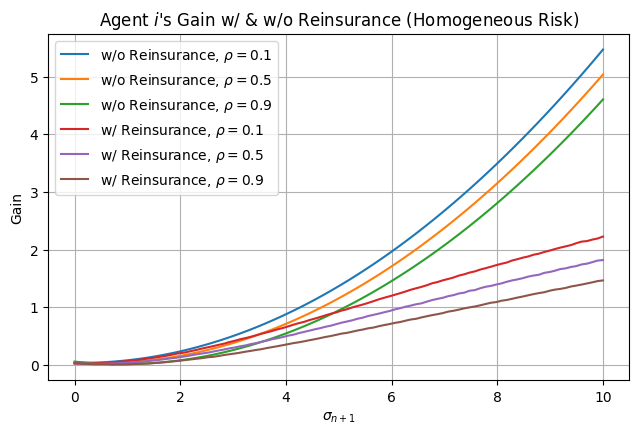
\includegraphics[width=\textwidth]{Figures/Equi_Gain_homo_rho.png}
%\subcaption{}
\label{fig:comparewwoR_equi_rho}
\end{subfigure}
\hfill
\begin{subfigure}[b]{0.45\textwidth}
\centering
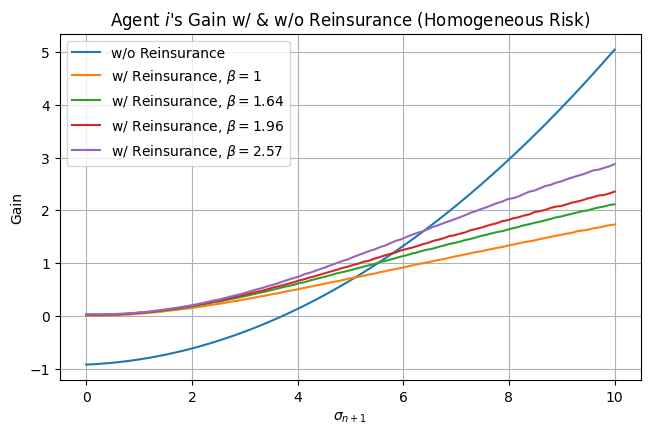
\includegraphics[width=\textwidth]{Figures/Equi_Gain_homo_beta.png}
%\subcaption{}
\label{fig:comparewwoR_equi_beta}
\end{subfigure}

\begin{subfigure}[b]{0.45\textwidth}
\centering
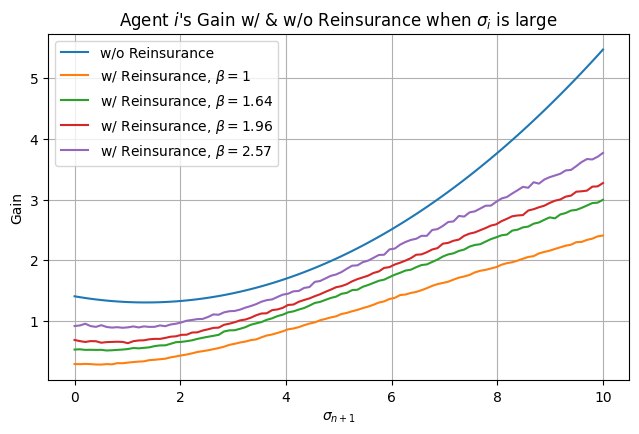
\includegraphics[width=\textwidth]{Figures/Equi_Gain_hete_ownbig.png}
%\subcaption{}
\label{fig:comparewwoR_equi_mybig}
\end{subfigure}
\hfill
\begin{subfigure}[b]{0.45\textwidth}
\centering
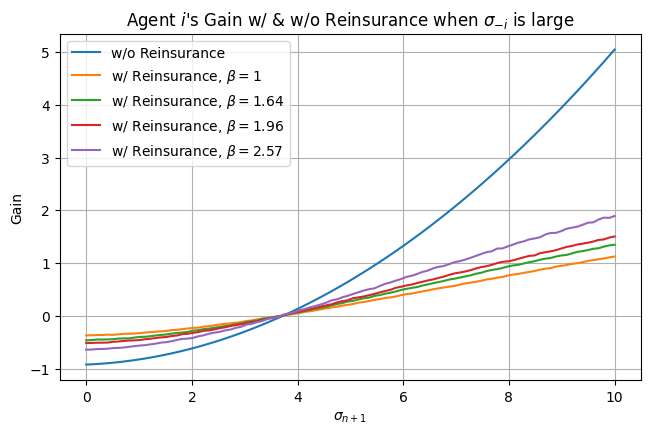
\includegraphics[width=\textwidth]{Figures/Equi_Gain_hete_otherbig.png}
%\subcaption{}
\label{fig:comparewwoR_equi_youbig}
\end{subfigure}
\noindent\begin{minipage}{\textwidth}
\raggedright
\NOTE{\\{\it Note}: SC occurs when the function is positive. In the homogeneous case, the fixed variance $\sigma^2=1,$ risk tolerance $\delta=1,$ reinsurance level $\beta=1.96$, and correlation $\rho=0.2$ are used, if it is not specified in the graph. In the heterogeneous case, the fixed risk tolerance $\delta=1,$ reinsurance level $\beta$, and correlation $\rho=0.2$ are used, if it is not specified in the graph. $\sigma^2_{high}=15$ is used for the higher variance, and $\sigma^2_{low}=1$ is used for the lower variance.}
\end{minipage}
\label{fig:comparewwoR_equi}
\end{figure}

A general observation on the MC simulation is that reinsurance decreases the gain of existing members due to the high risk of the candidate. This is indeed expected, as we have already emphasized, benefits from the reinsurance are higher for high-risk agents. Without reinsurance, the role of covering the high risk for a premium is assumed by existing members with relatively low risk. When the reinsurer is involved, it covers the aggregate risk above the level $K$ which includes part of the candidate's high risk. This reduces the premium paid to low-risk members and hence reduces their gains from sharing (due to lower cash compensation).   {As shown in the top-left and top-right panels of Figure \ref{fig:comparewwoR_equi}}, higher $\sigma_{n+1}$, higher correlation, and   {greater} reinsurance coverage   {reduce} gains for each   {existing (homogeneous)} member.   {Similarly, the bottom-left and bottom-right panels illustrate} that reinsurance   {diminishes} the benefits   {of pool} expansion for both high- and low-risk existing members.
% In fact, as pictured in Figures \ref{fig:comparewwoR_equi_rho} and \ref{fig:comparewwoR_equi_beta}, higher $\sigma_{n+1}$, higher correlation and higher reinsurance coverage yield lower gains for each (homogeneous) existing member.   

% By comparing Figures \ref{fig:comparewwoR_equi_mybig} and \ref{fig:comparewwoR_equi_youbig}, we observe that reinsurance reduces benefits for the pool's expansion for both high- and low-risk members in the original pool.

\subsubsection*{The effect of reinsurance on the acceptance region and gains}
Under FP, reinsurance does not change the acceptance region but changes the level of risk. This is illustrated   {on the left panel} in Figure \ref{fig:ARchange_fair_ep}, where the acceptance region for the existing member stays the same (interval of $\sigma_{n+1}$ that makes functions positive) but the gains (in the acceptance region), and the losses (in the rejection region) from the pool's expansion are lower under the reinsurance. In contrast, under EP, both the acceptance region and the gain change with the reinsurance.   {On the right panel} in Figure \ref{fig:ARchange_fair_ep}, the lower bound of $A$ is higher with reinsurance, which means that existing members are less willing to accept a candidate.
\begin{figure}[t]
\caption{Gain of an agent $i$ from the entrance without and with reinsurance ($\beta=1.96$), under the fairness and equilibrium principle.}
\centering
\begin{subfigure}[b]{0.45\textwidth}
\centering
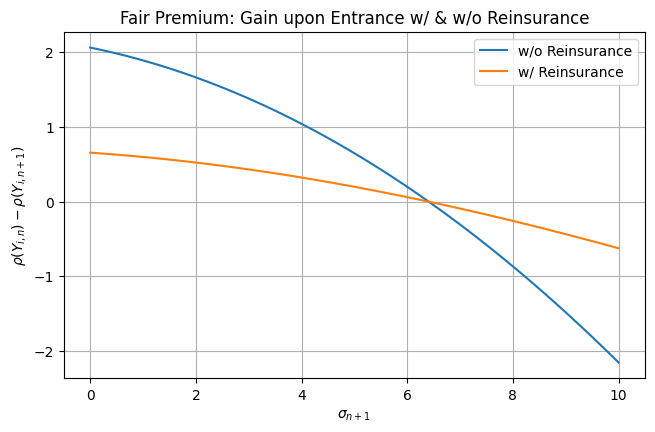
\includegraphics[width=\textwidth]{Figures/Fair_Gain_wwo_Rein.png}
% \subcaption{}
% \label{fig:fairchange}
\end{subfigure}
\hfill
\begin{subfigure}[b]{0.45\textwidth}
\centering
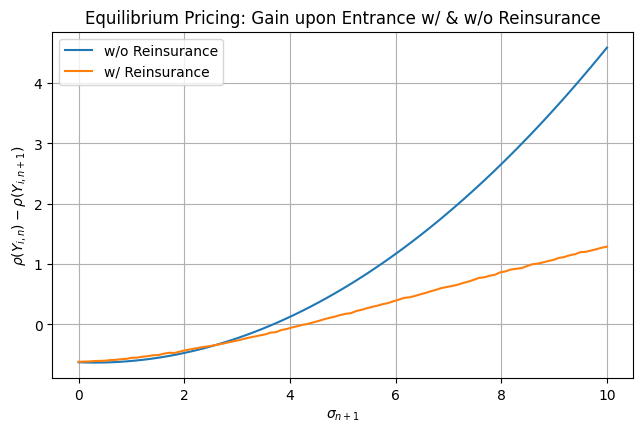
\includegraphics[width=\textwidth]{Figures/Equi_Gain_wwo_Rein.png}
% \subcaption{}
% \label{fig:ARchange}
\end{subfigure}
\label{fig:ARchange_fair_ep}
\end{figure}
Based on the above-simulated counter-example we estimate that
\begin{remark}
Unlike FP, the acceptance region becomes narrower with the reinsurance under EP.
\end{remark}
  {A simplified example that highlights the effect of reinsurance under EP is given in Appendix G.2% \ref{app:eg:EP_rein}
.} In conclusion, the equilibrium pricing guarantees stability and WC in any pool, while any existing pool accepts candidates with sufficiently high-risk positions (due to the associated high compensation). SC is also possible with lower and medium values of $\sigma_{n+1}$, while the reinsurance makes SC less likely for existing members.

\section{Two Indicative Case Studies}
\label{sec:discussion}

In this section, we complement the theoretical analysis by delving into two case studies of risk-sharing schemes. The first case entails the application of the framework to a real risk pool, namely the expansion of the Caribbean Catastrophe Risk Insurance Facility (CCRIF) to three Central American candidate countries. In the second case, we explore a hypothetical scenario of a health share among China's metropolitan areas. Our objective is to show how the model can be applied to real risk-sharing situations and to elucidate the decision-making process regarding the expansion of risk pools using real datasets. Note also that thanks to the robust analysis regarding the risks' distribution (see Section \ref{sec:conclusion} and Appendix C), general insights from these case studies could be qualitatively reliable even if the risks do not follow a normal distribution. Therefore, we could highlight the managerial and policy implications of our theoretical findings.


\subsection{Caribbean Catastrophe Risk Insurance Facility}
As mentioned in the introduction, the Caribbean Catastrophe Risk Insurance Facility (CCRIF) functions as a regional cooperative mechanism with the primary goal of safeguarding its member states from the economic fallout of natural disasters. Established in 2007 with 16 founding states, the CCRIF has steadily expanded its membership, now encompassing not only Caribbean nations but also others from Central America. The progression of membership since 2007 is detailed in Table \ref{tab:evolution}. These expansions are anticipated to bring mutual benefits to both existing (\textit{i.e.} SC) and new members by reducing premiums through more effective capital utilization and by diversifying the geographical coverage of the CCRIF portfolio. Besides providing a plain method to apply our framework to a rather complex situation, we aim to examine up to what extent the aforementioned assertions hold under the different imposed pricing rules. 
\begin{table}[t]
\centering
\caption{CCRIF Membership Evolution by Year from 2007 to 2023}
\begin{adjustbox}{width=\textwidth}
\begin{tabular}{rc}
\toprule\toprule
 Year & Members \\
\midrule
\multirow{3}{*}{2007} & Anguilla, Antigua and Barbuda, The Bahamas, Barbados, Belize, Bermuda, Cayman Islands,\\
&   Dominica, Grenada, Haiti, Jamaica, Saint Kitts and Nevis, Saint Lucia,\\
&Saint Vincent and the Grenadines, The Republic of Trinidad and Tobago, The Turks and Caicos Islands \\
2015 &   Nicaragua \\
2018 &  British Virgin Islands, Montserrat, Sint Maarten, Panama \\
2019 &  Guatemala  \\
2023 & Honduras\\
\bottomrule\bottomrule
\end{tabular}
\end{adjustbox}
\label{tab:evolution}
\end{table}

The operational framework of CCRIF is described in details in Appendix A.1. In short, similarly to our model, CCRIF collects premiums from its members and manages their aggregated risks by retaining a portion and transferring the remainder to reinsurance coverage (provided by a syndicate of companies). In other words, it is an excellent example of a risk pool that started with a specific founding members and has a standing aim to expand.  

Although, there are some operational differences between the CCRIF and our risk-sharing scheme (e.g. the payouts are determined by predetermined parameters or triggers and not by actual damages), there are substantial similarities regarding the way the risks are mutually shared and the induced members' benefits, making the CCRIF a rather indicative case study of our theoretical thesis. 

One could argue that the assumption of a competitive risk-sharing structure is weak, as large countries—whether currently participating in the pool or not—may behave strategically when sharing their risks. Although there is no evidence of such strategic behavior during CCRIF’s expansions, we cannot entirely dismiss the possibility. That said, because the catastrophic risks being pooled are publicly observable, any opportunity for strategic manipulation is likely limited to the premium structure. While large countries may exert some market power in influencing premiums, we believe this does not significantly affect the core insights or conclusions of our paper.

In order to apply the model, we need first to estimate the parameters of each county' risk. For this, we use the payout data of the CCRIF from 2007 to 2024 for all participating countries, which is publicly available on the CCRIF's website (\cite{ccrif_payouts}). To simplify the analysis, we consider only one source of catastrophic events, namely tropical cyclones. 

It is important to point out that under both pricing rules, there is no need to estimate the mean loss of individual country (only the aggregate mean is needed for SC conditions with reinsurance and EP). We need however to estimate the individual risks' variances, whereas the available data are not sufficient for all countries. In order to provide some reasonable estimation, we first estimate the mean $\hat{m}_n$ and the variance $\hat{s}_n^2$ of the aggregate annual risk (using all the aggregate data). Then, we apply a proxy (based on the indicator random variable) to estimate each country's variance: $\text{Adjusted\_Variance}_i =\hat{\sigma}_i^2:= k^2 \times \left(\text{Occurrence\_Probability}_i\right)\times \left(1-\text{Occurrence\_Probability}_i\right) \times \left(\text{GDP}_i\right)^2$, where $k$ is the (unique) constant that makes the sum of adjusted variances and the variance of total loss equal, under the fixed pairwise correlation assumption: $\sum_{j}\hat{\sigma}_j^2+2\rho\sum_{i\neq j}\hat{\sigma}_i\hat{\sigma}_j= \hat{s}_n^2$. As for the correlation, in the main scenarios we consider two modest choices $\rho=0.1$ and $\rho=0.3$. Details with regard to parameters for each country are summarized in Appendix A.2. Furthermore, while the analysis could be done with different risk tolerances, we choose to work with common ones ($\delta_i=1$, for each $i$), in order to focus solely on their riskiness. 

The next step is to impose a group of countries as the existing risk pool, which is an essential component of our framework. For this, we follow the history of CCRIF and consider its founding members as the existing ones. Subsequently, British Virgin Islands, Nicaragua, Panama and Guatemala are considered as candidates whose risk profiles are summarized in Table \ref{tab:CCRIF_summary}. One would expect that any of these pool expansions is going to be beneficial for each existing member because of the induced wider sharing. However, the model suggests that expansion does not always improve existing members' risk measures even when the correlation is low, \textit{i.e.} SC may not hold. In particular, under FP, the expansion with members with high DTR, such as Guatemala, Nicaragua, and Panama (each exhibiting significantly higher DTRs than the existing pool) worsens existing members' risks. Table \ref{tab:CCRIF_summary} states the exact levels of DTR that the expansion has to meet in order to reach SC. 

Conversely, if EP is applied, countries with relatively low riskiness such as the British Virgin Islands, Nicaragua, and Panama violate the SC. Results for SC are visualized in Table \ref{tab:CCRIF_summary}. We point out that under FP, even with low correlation of risks only a country with sufficiently low DTR leads to SC (even when correlation is low). On the other hand, under EP the SC is reached in the expansion with high DTR countries, the number of which increases when the correlation of risks becomes lower. In fact, we have verified that the checkmarks of Table \ref{tab:CCRIF_summary} remain the same when the correlation increases to $0.5$.  


%These possible expansions are anticipated to benefit both existing and new members due to their geographical diversity. For instance, Central America faces a higher exposure to earthquakes compared to the Caribbean, as it lies within the ‘Ring of Fire,’ a region along the Pacific Ocean known for its active volcanoes and frequent earthquakes.
\begin{figure}[t]
\centering
\begin{minipage}{0.44\textwidth}
\centering
\caption{Geographic location of CCRIF countries and candidates considered in this case study}
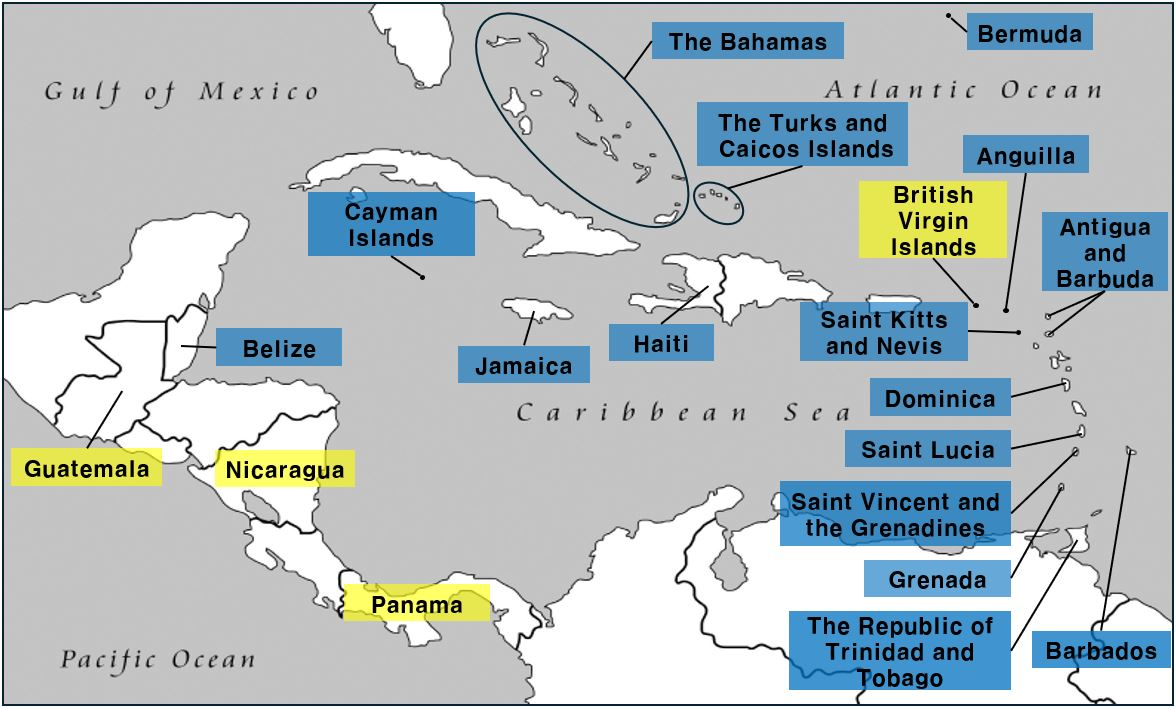
\includegraphics[width=\textwidth]{Figures/map_CCRIF_corrected.JPG}
\label{fig:ct-america}
\end{minipage}
\hfill
\begin{minipage}{0.55\textwidth}
\centering
\captionof{table}{Summary of statistics and decision-making for the expansion of CCRIF (checkmark refers to SC)}
\begin{adjustbox}{width=\textwidth}
\begin{tabular}{l|cc|cccc|cccc}
\hline\hline
\multirow{3}{*}{}      & \multicolumn{2}{c|}{\multirow{2}{*}{DTR}} & \multicolumn{4}{c|}{W/O Reinsurance}    & \multicolumn{4}{c}{W/ Reinsurance} \\ 

\cline{4-11} 
& \multicolumn{2}{c|}{}  & \multicolumn{2}{c|}{FP} & \multicolumn{2}{c|}{EP}    & \multicolumn{2}{c|}{FP} & \multicolumn{2}{c}{EP}      \\ 

\cline{1-11} Pairwise correlation 
& \multicolumn{1}{c|}{0.1}      & 0.3& \multicolumn{1}{c|}{0.1}    & \multicolumn{1}{c|}{0.3}    & \multicolumn{1}{c|}{0.1}    & 0.3    & \multicolumn{1}{c|}{0.1}    & \multicolumn{1}{c|}{0.3}    & \multicolumn{1}{c|}{0.1}    & 0.3 \\ 

\hline\hline
Existing Pool   & \multicolumn{1}{c|}{1.02}  & 0.99      & \multicolumn{1}{c|}{-} & \multicolumn{1}{c|}{-} & \multicolumn{1}{c|}{-} & - & \multicolumn{1}{c|}{-} & \multicolumn{1}{c|}{-} & \multicolumn{1}{c|}{-} & -   \\ \hline

British Virgin Islands & \multicolumn{1}{c|}{0.04}  & 0.03      & \multicolumn{1}{c|}{\checkmark} & \multicolumn{1}{c|}{\checkmark} & \multicolumn{1}{c|}{}  &   & \multicolumn{1}{c|}{\checkmark} & \multicolumn{1}{c|}{\checkmark} & \multicolumn{1}{c|}{}  &     \\ \hline

Guatemala  & \multicolumn{1}{c|}{23.04}  & 17.39     & \multicolumn{1}{c|}{}  & \multicolumn{1}{c|}{}  & \multicolumn{1}{c|}{\checkmark} & \checkmark & \multicolumn{1}{c|}{}  & \multicolumn{1}{c|}{}  & \multicolumn{1}{c|}{\checkmark} &     \\ \hline

Nicaragua  & \multicolumn{1}{c|}{6.67}  & 5.03      & \multicolumn{1}{c|}{}  & \multicolumn{1}{c|}{}  & \multicolumn{1}{c|}{\checkmark} &   & \multicolumn{1}{c|}{}  & \multicolumn{1}{c|}{}  & \multicolumn{1}{c|}{\checkmark} &     \\ \hline

Panama     & \multicolumn{1}{c|}{7.76}  & 5.85      & \multicolumn{1}{c|}{}  & \multicolumn{1}{c|}{}  & \multicolumn{1}{c|}{\checkmark} &   & \multicolumn{1}{c|}{}  & \multicolumn{1}{c|}{}  & \multicolumn{1}{c|}{\checkmark} &     \\ \hline\hline
\end{tabular}
\end{adjustbox}
\label{tab:CCRIF_summary}
\end{minipage}
\end{figure}
The model also verifies that when the EP is considered, the presence of reinsurance reduces the benefits of riskier new entrances, since the premium is shared with the reinsurer. In fact, for higher correlations, SC does not hold for none of the candidates. We therefore have a situation where the effect of pool expansion could be negative for the some of the existing members, with the imposed pricing rule being the determinant factor. On the other hand, when the aggregate welfare is considered, WC is the appropriate property to study. By construction, EP guarantees WC with and without reinsurance, while under FP countries with low DTR may want to leave the pool, especially when correlation of risks is not sufficiently low. In fact,  CCRIF’s actual expansion is consistent with our model’s prediction under
the EP, since the guaranteed WC suffices to allow expansion (absent a veto
rule), even for relatively riskier countries.
Although we do not claim that
CCRIF strictly applies EP, our model predicts that any expansion involving riskier entrants would necessarily involve a risk premium shared among existing members. 


In summary, the case of CCRIF exemplifies a scenario where our theoretical framework offers essential guidance, enabling the alignment of desired expansion outcomes with the corresponding risk-pool design. Furthermore, it offers concrete managerial insights into pool expansion by demonstrating how different pricing rules lead to varying consensus outcomes using real data, and by emphasizing the impact of reinsurance on individual welfare.





%This case study demonstrates that certain expansions may have adversely affected the standing of the existing pool, challenging the simplistic assumption that diversification would invariably enhance the situation for current members. Instead of relying solely on intuition, our model provides a structured approach that quantifies the impact of expansion, thereby supporting informed decision-making and offering valuable insights for expansion strategies. Moreover, the findings underscore the potential advantages of embracing premium rules other than FP, such as EP. While it can be argued that all known risk pools in practice today are based on EP, the FP allows for the possibility of a larger pool compared to EP. This strategy may likely be pursued by unions of members with substantial wealth seeking higher premiums in exchange for assuming increased risk.

\subsection{Potential Healthcare Sharing in China}

China's national healthcare insurance program is administered at the municipality and provincial levels, presenting local governments with numerous challenges, particularly in light of escalating medical costs and a rapidly aging population. A way to deal with these issues is by healthcare sharing. This is a risk-share pool concept, prevalent in many countries, that enables participants to collectively manage medical expenses. In this section, we construct a hypothetical example demonstrating the establishment of a risk pool among major metropolitan regions in China and apply and examine our expansion notions.  

For this, we got access to a unique dataset pertaining to healthcare services and insurance claims within China’s health insurance system for the year 2020. This dataset encompasses various information, including gender, date of birth, visited hospital names, medical conditions or diagnoses, and the financial reimbursement amounts provided under insurance claims. Data was aggregated by cities based on individuals' hospital visits, enabling the estimation of risk's parameters across different urban centers. Further specifics about the dataset and details about the parameters' estimation are provided in Appendix B.1.% \ref{app:health_data} and \ref{app:health_simul}.

Pooling risks across geographically diverse cities is again supposed to yield benefits through risk diversification. For instance, Shanghai experiences higher humidity levels than many other cities due to its proximity to the Yangtze River Delta and the East China Sea, combined with its dense urban environment. These conditions influence the prevalence and severity of asthma symptoms, which in turn affect health insurance claims. Pooling such geography-specific risks across various cities is expected to generate more favorable risk profiles for all involved cities in a SC sense. Our goal is apply our framework and examine whether this conjecture holds. 

\begin{figure}[t]
\centering
\begin{minipage}{0.44\textwidth}
\centering
\caption{A hypothetical expansion of healthcare sharing in China}
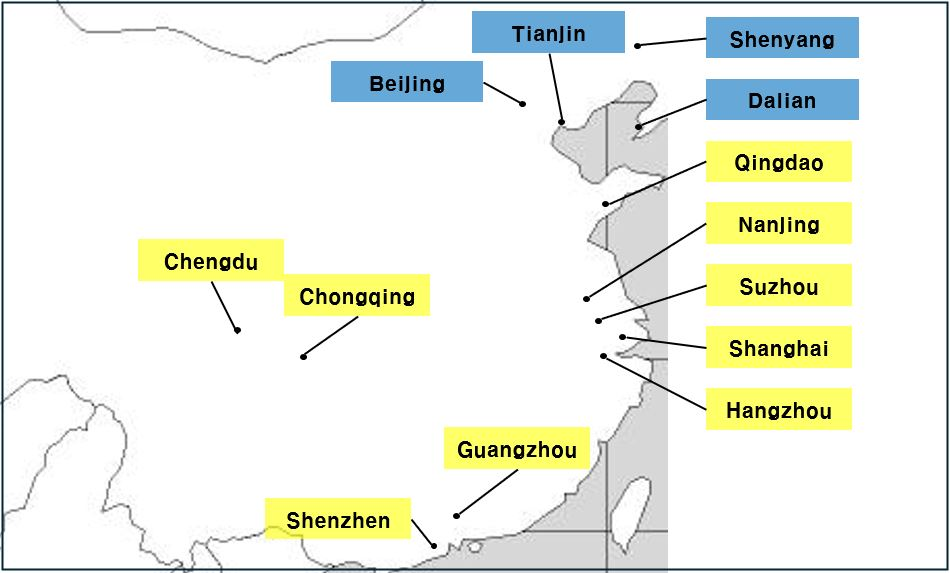
\includegraphics[width=\textwidth]{Figures/map_china.JPG}
\label{fig:china-america}
\end{minipage}
\hfill
\begin{minipage}{0.55\textwidth}
\centering
\captionof{table}{Summary of statistics and expansion of healthcare sharing (checkmark refers to SC)}
\begin{adjustbox}{width=\textwidth}
\begin{tabular}{l|c|cc|cc}
\hline\hline
&     & \multicolumn{2}{c|}{W/O Reinsurance}                                       & \multicolumn{2}{c|}{W/ Reinsurance}                                        \\ \hline
& DRT & \multicolumn{1}{c|}{Fairness}                  & Equilibrium               & \multicolumn{1}{c|}{Fairness}                  & Equilibrium               \\ \hline\hline
Existing pool &    2.9 & \multicolumn{1}{c|}{-}                         & -                         & \multicolumn{1}{c|}{-}                         & -                         \\ \hline
Chengdu       &   1.92  & \multicolumn{1}{c|}{\checkmark} &  \multicolumn{1}{c|}{\checkmark}                         & \multicolumn{1}{c|}{\checkmark} &                           \\ \hline
Chongqing     &   3.11  & \multicolumn{1}{c|}{\checkmark} &    \multicolumn{1}{c|}{\checkmark}                       & \multicolumn{1}{c|}{\checkmark} &                          \\ \hline
Guangzhou     &    5.64 & \multicolumn{1}{c|}{}                          & \checkmark & \multicolumn{1}{c|}{}                          & \checkmark \\ \hline
Qingdao       &   3.14  & \multicolumn{1}{c|}{\checkmark} &     \multicolumn{1}{c|}{\checkmark}                      & \multicolumn{1}{c|}{\checkmark} &                           \\ \hline
Shanghai      &   3.03  & \multicolumn{1}{c|}{\checkmark} &    \multicolumn{1}{c|}{\checkmark}                       & \multicolumn{1}{c|}{\checkmark} &                           \\ \hline
Shenzhen      &    3.11 & \multicolumn{1}{c|}{\checkmark} &    \multicolumn{1}{c|}{\checkmark}                       & \multicolumn{1}{c|}{\checkmark} &                           \\ \hline
Others        & -    & \multicolumn{1}{c|}{\checkmark} & \checkmark & \multicolumn{1}{c|}{\checkmark} & \checkmark \\ \hline\hline
\end{tabular}
\end{adjustbox}
\noindent\begin{minipage}{\textwidth}
\raggedright
\NOTE{\\\smallskip{\footnotesize{\it Note}: 'Others' includes Hangzhou, Nanjing, and Suzhou.}}
\end{minipage}
\label{tab:HI_summary}
\end{minipage}
\end{figure}
% \begin{table}[t]
% \centering
% \caption{Health Insurance: Summary of Expansion}
% \begin{tabular}{lcc}
% \hline\hline
% \textbf{Acceptance} & \textbf{Fairness Principle} & \textbf{Equilibrium Principle} \\
% \hline
% Without Reinsurance & All except Guangzhou& All cities accepted\\
% With Reinsurance    & All except Guangzhou & \begin{tabular}[c]{@{}c@{}}Excludes Chengdu, Chongqing,\\ Qingdao, Shanghai, Shenzhen\end{tabular} \\
% \hline\hline
% \end{tabular}
% \label{tab:expansion_insu}
% \end{table}

As the existing group we consider a pool of major cities in northeastern China, such as Beijing and Tianjin (labeled blue in Figure \ref{fig:china-america}). The objective is to consider the expansion to other regions, such as eastern coastal cities like Shanghai and Shenzhen (labeled yellow in Figure \ref{fig:china-america}). Similarly to the previous case study, we outline the expansion for different candidates under SC perspective in Table \ref{tab:HI_summary}. The main scenario sets the pairwise correlation equal to $\rho=0.3$.

Under the risk neutral pricing rule, \textit{i.e.} FP, the existing members will accept all candidate cities except Guangzhou due to its relatively high risk compared to the existing pool, regardless of whether reinsurance is applied. Under EP, however, all candidate cities are accepted without reinsurance. Introducing reinsurance makes the existing pool more selective, leading to the exclusion of cities such as Chengdu, as their lower risk levels fail to generate sufficient compensation to justify its inclusion.

We conducted the same analysis also with lower, $\rho=0.1$, and higher risks' correlation $\rho=0.5$. As expected, a decrease in pairwise correlation enhances diversification, allowing for example Guangzhou to join under FP with and without reinsurance. In contrast, at $\rho=0.5$, Hangzhou is not accepted under EP with reinsurance but continues to be accepted without it. Of course, the situation is different when WC is considered. EP yields WC and hence higher welfare (if there is no subgroup formation), whereas, entrance of regions with high DTR, such as Guangzhou, may force the cities with low DTR to leave the pool. 

Our theoretical framework could serve as a managerial guide for the design of new risk-sharing
pools, such as a healthcare-sharing. This hypothetical example offers interesting insights for decision-makers, on whether and how regional healthcare sharing should be formulated regarding premiums and reinsurance in order to get WC and SC.



\section{Conclusion and Other Distributions}\label{sec:conclusion}
\begin{table}[t]
\caption{Summary Table for Main Results.}
\centering
\resizebox{\textwidth}{!}{%
\begin{tabular}{|c|c|c|c|}
\toprule\toprule
&\multirow{2}{*}{\textbf{Type}}&\multicolumn{2}{c|}{\textbf{Reinsurance}}\\\cline{3-4}

&&\textbf{Without}&\textbf{With}\\
\toprule\multirow{3}{*}{\begin{tabular}{c}
\textbf{Fairness}\\
\textbf{Pricing}
\end{tabular} }&\textit{Stability} & Aggr(DRT) $\leq$ Ind(DRT)  & Wider \\\cline{2-4}
&\textit{Weak} & New Aggr(DRT) $\leq$ Ind(DRT) & Wider \\\cline{2-4}
&\textit{Strong} & New Aggr(DRT) $\leq \min\left\{\text{Old Aggr(DRT)},  \text{Cand(DRT)}\right\}$ & \begin{tabular}{c}
Same for exist.~members\\
\& wider for candidate
\end{tabular}\\
\hline
\multirow{3}{*}{\begin{tabular}{c}
\textbf{Equilibrium}\\
\textbf{Pricing}
\end{tabular}}&\textit{Stability} & Always &  Always\\\cline{2-4}

&\textit{Weak} & Always & Always\\\cline{2-4}
&\textit{Strong} & 
\begin{tabular}{c}
 Always for high $\sigma_{n+1}$\\ \& potentially for low and mid values of $\sigma_{n+1}$ 
\end{tabular}
& \begin{tabular}{c}
Narrower for exist.~members\\
\& same for candidate
\end{tabular}\\\toprule\toprule
\end{tabular}
}
\noindent\begin{minipage}{\textwidth}
\raggedright
\NOTE{\\\smallskip{\it Note}: DRT = Deviation/Tolerance ratio, Aggr = Aggregate, Ind = Individual, Old and New refer to before and after expansion.}
\end{minipage}
\label{tab:summary2}
\end{table}
   {This paper investigates an existing risk pool expansion by establishing two notions of existing members' consensus. The analysis employs entropic risk measures and considers two distinct pricing rules for risk transfers:} the fairness principle (FP) and the equilibrium principle (EP). The key findings can be summarized as follows. 1) Under both pricing rules, the decision for acceptance depends solely on the variance of the candidate's risk, disregarding the mean. 2) The acceptance decision by an existing member or a candidate under FP is exclusively based on DTR. 3) Low-risk candidates are more likely to be accepted under FP, whereas high-risk candidates are accepted only under risk-adjusted pricing such as the equilibrium one. 4) In the context of SC, reinsurance does not change the acceptance decision of existing members under FP. In contrast, under EP, a candidate is less likely to be accepted with a reinsurance. Furthermore, a candidate's willingness to join the risk pool remains unchanged with reinsurance under EP but increases under FP. 5) Reinsurance enhances the stability of the risk pool under FP, {\it i.e.}, members are less likely to leave the risk pool. 6) WC and stability conditions hold in any case both with and without reinsurance under EP. A summary of the main results in this paper can be found in Table \ref{tab:summary2}.    {Additionally, the paper analyzes two case studies of risk pools using real data through which the managerial insights of the models are highlighted.} 

The paper   {could} be further extended to   {explore} the effects of risk pooling   {in} several potential directions.   {For instance, one could implement} alternatives to the entropic risk measure, even under a linear (in that case) sub-optimal sharing rule and   {explore the potential} connection between the pool's properties regarding its expansion   {and} specific properties of pricing rules.   {Under a different perspective, we may investigate whether it might} be optimal for the members to form sub-groups rather than expanding or maintaining the existing group   {, consider possible delayed payments for cash transfers inside the pool and/or the reinsurance premium and apply the notions of WC and SC to other sharing environments, such as club theory. In a different direction, SC and WC could also be experimentally studied
in a similar manner as in the works of \cite{Ahlin20} and \cite{CarpeSadou00} on credit sharing and \cite{Rob12} and \cite{AmbMobSze14} on the sharing of household insurance.}

% \subsection{  {Other Distributions}} As a final note, we comment on a potential critique on the imposed joint normal distribution assumption. While normality substantially helps the deviation of explicit formulas and the presentation of the paper's contributions, it is not necessary for the 
% validity of the qualitative lessons of the paper. 

% In order to show it, we conduct a number of simulations to explore whether the managerial insights derived from previous sections hold true for distributions other than normal. Specifically, we examine three classes of well-known and widely-used distributions: exponential, Gamma, and Pareto. The details of these simulations and their outcomes are provided in Appendix C.
% % \ref{app:simulation}.

% The simulations demonstrate that the qualitative results remain untouched when the alternative distributions are imposed. Risk pools tend to exhibit conservative behavior under FP and become risk-seeking under EP. Across all three distributions, the existing pool showed a preference for candidates with lower risk under FP, while it favored candidates with higher risk under EP. Also, although entropic risk measures may not be applicable to certain distributions (such as Pareto), we consider finite sample estimates in order to capture the distributional characteristics. This consistency suggests that the conclusions are likely to extend to other distributions as well, despite the involved analytical complexities.

As a final note, we address a potential critique regarding the assumption of a joint normal distribution. It is known in the literature (e.g. \cite{CHEN2025100003}) that optimal risk sharing strategies for heavy-tailed distributions such as Pareto under various criteria can be quite different from those for light-tailed distributions such as normal. While the normality assumption significantly facilitates the derivation of explicit formulas and enhances the clarity of the paper's contributions, it is not essential for the validity of the qualitative insights presented.

To demonstrate this, we conducted a series of simulations to investigate whether the managerial insights derived in earlier sections hold true for distributions other than the normal distribution. Specifically, we examine three well-known and widely-used classes of distributions: exponential, Gamma, and Pareto. The details of these simulations and their results are provided in Appendix C.

The simulations reveal that the qualitative findings remain robust under these alternative distributions. Risk pools consistently exhibit conservative behavior under FP and risk-seeking behavior under EP. Across all three distributions, existing pools preferred candidates with lower risk under FP and favored those with higher risk under EP. Additionally, while entropic risk measures may not be directly applicable to certain distributions (such as Pareto), we can employ finite sample estimates to capture the essential characteristics of these distributions. This consistency suggests that the conclusions are likely to generalize to other distributions, despite the analytical complexities involved.

\section{Acknowledgment}

The authors gratefully acknowledge the financial support for this research provided by the Tsinghua University School of Economics and Management Research Grant (2023051001) and the National Social Sciences Foundation of China Major Grant (23\&ZD178).


% References here (outcomment the appropriate case)


% \begin{appendices}


%  { \iffalse

% \section{Proof of Theorem \ref{thm:finite} \label{proof:finitewcs} }
% Let us eliminate all the adjustable variables in $\mathcal{X}$ via Algorithm \ref{alg:FME}, and we have 
% \begin{equation*}
% \mathcal{X}_{\setminus [N_2]} =  \left\{ \mb{x} \in X \hspace{3pt} | \hspace{3pt} \mb{G}(\mb{z}) \mb{x}  \geq\mb{h}(\mb{z})  \quad  \forall \mb{z} \in \mathcal{W} \right\},
% \end{equation*}

% 	where $\mb{G}\in \mathcal{L}^{I_1,M_G}$ and $M_G \in \mathbb{Z}_+$ denotes the number of constraints. Suppose the semi-infinite constrained set $\mathcal{X}_{\setminus [N_2]}$ admits the following tractable counterpart (see, e.g., \cite{bdv15,gbbd14}):
% \begin{equation*}
% 	\mathcal{X}^{c}_{\setminus [N_2]} =\left\{ \mb{x} \in X \enskip | \enskip \exists \mb{\omega} \ge \mb{0}: \enskip f_i(\mb{x}, \mb{\omega}) \le 0 \enskip \forall i\in [M_c] \right\}
% \end{equation*}
% 	where the functions $f_i$, $\forall i\in [M_c]$, that are affine in $\mb{x}$ and convex in the dual (auxiliary) variables $\mb{\omega}$. The set $\mathcal{X}^{c}_{\setminus [N_2]}$ is an equivalent convex representation of $\mathcal{X}_{\setminus [N_2]}$, and
% \begin{equation} \label{eq:convexref}
% 	\min_{\boldsymbol{x} \in \mathcal{X}} \mb{c}'\mb{x} =\min_{\boldsymbol{x} \in \mathcal{X}_{\setminus [N_2]}} \mb{c}'\mb{x} = \min_{\boldsymbol{x} \in \mathcal{X}^{c}_{\setminus [N_2]}} \mb{c}'\mb{x}.
% \end{equation}

%     Let us denote $(\mb{x}^*,\mb{\omega}^*)$ as an optimal solution of the convex optimization problem in $(\ref{eq:convexref})$, and partition the constraints in $\mathcal{X}^{c}_{\setminus [N_2]}$ into two subsets: 
% \begin{equation*}
% 	f_i^b(\mb{x}^*,\mb{\omega}^*) = 0  \quad \forall i\in [M^b_c], \quad f_i^n(\mb{x}^*,\mb{\omega}^*) <0  \quad \forall i\in [M^n_c].
% \end{equation*}
% 	Note that $f_i^b(\mb{x},\mb{\omega}^*), \forall i\in [M^b_c]$, and $f_i^n(\mb{x},\mb{\omega}^*)$,  $\forall i\in [M^n_c]$,  are affine in $\mb{x}$. Since $\mb{x} \in \mathbb{R}^{N_1}$, there are at most $N_1$ linearly independent equalities among $f_i^b(\mb{x},\mb{\omega}^*) = 0$, $\forall i\in [M^b_c]$.  Let us represent the (at most $N_1$) linearly independent equalities as a linear system $A\mb{x} = \mb{b}$, for some matrices $A$ and vectors $\mb{b}$. Since $\mb{x}^* \in \left\{ \mb{x} \,| \, A\mb{x} = \mb{b} \right\}$,  we have $\min_{\boldsymbol{x} : A\boldsymbol{x} = \boldsymbol{b} } \mb{c}'\mb{x} \le \mb{c}'\mb{x}^*$. We now show that $\min_{\boldsymbol{x} : A\boldsymbol{x} = \boldsymbol{b} } \mb{c}'\mb{x} = \mb{c}'\mb{x}^*$ by contradiction.	Suppose there exists a $\overline{\mb{x}} \in \left\{ \mb{x} \,| \, A\mb{x} = \mb{b} \right\}$, such that $\mb{c}'\overline{\mb{x}} < \mb{c}'\mb{x}^*$. Then, there exists a $\mb{x}^{\dagger} = \theta \overline{\mb{x}} +(1- \theta)\mb{x}^* \in \left\{ \mb{x} \,| \, A\mb{x} = \mb{b} \right\}$, $\theta\in (0,1]$, such that the non-binding constraints remain non-binding,{\it i.e.}, $f_i^n(\mb{x}^{\dagger},\mb{\omega}^*) <0 , \forall i\in [M^n_c]$, and $ \mb{c}'\mb{x}^{\dagger} < \mb{c}'\mb{x}^*$, which contradicts with the optimality of $\mb{x}^*$.  Hence, $\min_{\boldsymbol{x} : A\boldsymbol{x} = \boldsymbol{b} } \mb{c}'\mb{x} = \mb{c}'\mb{x}^*$. 

% 	Each linearly independent equality in $A\mb{x}^* = \mb{b}$ corresponds to (at least) one worst-case scenario in $\mathcal{X}_{\setminus [N_2]}$, and each worst-case scenario is the dual variable of $\mb{w}^*$, which can be easily determined from the KKT conditions. Let $\widehat{\mathcal{W}}$ be a set that contains one worst-case scenario from each equality of $A\mb{x}^* = \mb{b}$,{\it i.e.}, $|\widehat{\mathcal{W}}| \le N_1$, we have
% \begin{equation} \label{set:finitewcs}
% 	\begin{aligned}
% 	\left\{ \mb{x} \, | \,  A\mb{x} = \mb{b} \right\}   \supseteq& \left\{ \mb{x} \in X  \enskip | \enskip  \boldsymbol{G}(\boldsymbol{z}) \boldsymbol{x}  \ge \boldsymbol{f} (\boldsymbol{z}) \enskip \forall \boldsymbol{z} \in  \widehat{\mathcal{W}} \right\}\\
% 	=&  \left\{ \mb{x} \in X  \enskip |  \enskip \exists \mb{y} \in \mathcal{R}^{I_1,N_2}: \mb{A}(\mb{z}) \mb{x}+\mb{B}\mb{y}(\mb{z}) \geq\mb{d}(\mb{z})  \enskip \forall \mb{z} \in  \widehat{\mathcal{W}} \right\}\\
% 	=&  \mathcal{X}^{\dagger}.
% 	\end{aligned}
% \end{equation}
% 	The first line of (\ref{set:finitewcs}) holds because the worst-case scenarios $\mb{z} \in \widehat{\mathcal{W}}$ ensure that the equalities $A\mb{x} = \mb{b}$ are satisfied; the set equality (the second line of (\ref{set:finitewcs})) holds due to Theorem \ref{thm:equivalence}. Since  $\mb{x}^* \in \mathcal{X}^{\dagger}$, we have
% 	$
% 	\mb{c}'\mb{x}^* = \min_{\boldsymbol{x} : A \boldsymbol{x} = \boldsymbol{b}} \mb{c}'\mb{x} = \min_{\boldsymbol{x} \in \mathcal{X}^{\dagger}} \mb{c}'\mb{x}.
% 	$ \hfill \Halmos
% \fi

% }

% 	\section{Proof of } 
% \end{appendices}	

% \newpage

% Acknowledgments here
% \ACKNOWLEDGMENT{The authors are grateful to the associate editor and two anonymous referees for valuable comments on an earlier version of the paper. The research of the first author is supported by NWO Grant 613.001.208. The third author acknowledges the funding support from the Singapore Ministry of Education Social Science Research Thematic Grant MOE2016-SSRTG-059. Disclaimer: Any opinions, findings, and conclusions or recommendations expressed in this material are those of the author(s) and do not reflect the views of the Singapore Ministry of Education or the Singapore Government.}	

\bibliography{bibliography}
% CASE 1: BiBTeX used to constantly update the references
%   (while the paper is being written).
%\bibliographystyle{ormsv080} % outcomment this and next line in Case 1
%\bibliography{<your bib file(s)>} % if more than one, comma separated

% CASE 2: BiBTeX used to generate mypaper.bbl (to be further fine tuned)
%\input{mypaper.bbl} % outcomment this line in Case 2

%If you don't use BiBTex, you can manually itemize references as shown below.

%\newpage

% \begin{thebibliography}{}%
% 			\bibitem[{Ardestani-Jaafari and Delage(2016a)}]{ad16a}
% 			Ardestani-Jaafari, A., E. Delage (2016a)
% 			Linearized robust counterparts of two-stage robust optimization problems with applications in operations management. Available at: { \url{optimization-online.org/DB_FILE/2016/03/5388.pdf}}.
        
% 			\bibitem[{Ardestani-Jaafari and Delage(2016b)}]{ad16b}
% 			Ardestani-Jaafari, A., E. Delage (2016b)
% 			Robust optimization of sums of piecewise linear functions with application to inventory problems.  {\it Operations Research} 64(2):474--494.

% 			\bibitem[{Bemporad et~al.(2003)}]{bbm03}
% 			Bemporad, A., F. Borrelli, M. Morari (2003)
% 			Min-max control of constrained uncertain discrete-time linear systems.
% 			{\it IEEE Transactions Automatic Control} 48(9):1600--1606.	

% 			\bibitem[{Ben-Ameur et~al.(2016)}]{bwoz16}
% 			Ben-Ameur, W., G. Wang, A. Ouorou, M. Zotkiewicz  (2016)
% 			Multipolar Robust Optimization. Available at: { \url{arxiv.org/pdf/1604.01813.pdf}}.	

        
% 			\bibitem[{Ben-Tal et~al.(2009)}]{ben09}
% 			Ben-Tal, A., L. El Ghaoui,   A. Nemirovski (2009)
% 			{\it Robust Optimization}.
% 			Princeton Series in Applied Mathematics (Princeton University Press, Princeton, NJ).

% 			\bibitem[{Ben-Tal et~al.(2015)}]{bdv15}
% 			Ben-Tal, A., D. den Hertog, J.P. Vial (2015)
% 			Deriving robust counterparts of nonlinear uncertain inequalities.
% 			{\it Mathematical Programming} 149(1):265--299.


% 			\bibitem[{Ben-Tal et~al.(2016)}]{beg16}
% 			Ben-Tal, A., O. El Housni, V. Goyal (2016)
% 			A tractable approach for designing piecewise affine policies in dynamic robust optimization. Available at: \url{optimization-online.org/DB_FILE/2016/07/5557.pdf}.

        
% 			\bibitem[{Ben-Tal et~al.(2004)}]{bggn04}
% 			Ben-Tal, A., A. Goryashko, E. Guslitzer, A. Nemirovski (2004)
% 			Ajustable robust solutions of uncertain linear programs. {\it Mathematical Programming} 99:351--376.

% 			\bibitem[{Ben-Tal and Nemirovski(1998)}]{bn98}
% 			Ben-Tal, A., A. Nemirovski (1998)
% 			Robust convex optimization. {\it Mathematics of Operations Research} 23(4):769--805.

% 			\bibitem[{Ben-Tal and Nemirovski(1999)}]{bn99}
% 			Ben-Tal, A., A. Nemirovski (1999)
% 			Robust solutions of uncertain linear programs. {\it Operations Research Letters} 25:1--13.

% 			\bibitem[{Ben-Tal and Nemirovski(2000)}]{bn00}
% 			Ben-Tal, A., A. Nemirovski (2000)
% 			Robust solutions of linear programming problems contaminated with uncertain data. {\it Mathematical Programming} 88(3):411--424.


% 			\bibitem[Bertsimas and Brown(2009)]{bb09}
% 			Bertsimas, D., D. Brown (2009)
% 			Constructing uncertainty sets for robust linear optimization. {\it Operations Research} 57(6):1483--1495.

% 			\bibitem[Bertsimas et~al.(2011)]{bbc11}
% 			Bertsimas, D.,  D. Brown,  C. Caramanis (2011).
% 			Theory and applications of robust optimization. {\it SIAM Review}, 53(3):464--501.


% 			\bibitem[Bertsimas and Caramanis(2010)]{bc10}
% 			Bertsimas, D.,   C. Caramanis (2010).
% 			Finite adaptability for linear optimization. {\it IEEE Transactions on Automatic Control}, 55(12):1751--2766.

% 			\bibitem[{Bertsimas and Dunning(2016)}]{bd16a}
% 			Bertsimas, D., I. Dunning (2016)
% 			Multistage robust mixed integer optimization with adaptive partitions.  {\it Operations Research} 64(4):980--998.

% 			\bibitem[{Bertsimas et~al.(2015)}]{bdl15}
% 			Bertsimas, D., I. Dunning, M. Lubin (2015)
% 			Reformulation versus cutting-planes for robust optimization.  {\it Computational Management Science} 13(2):195--217.


% 			\bibitem[{Bertsimas and Georghiou(2015)}]{bg15}
% 			Bertsimas, D., A. Georghiou (2015)
% 			Design of near optimal decision rules in multistage adaptive mixed-integer
% 			optimization. {\it Operations Research} 63(3):610--627.		

% 			\bibitem[{Bertsimas and Goyal(2012)}]{bg12}
% 			Bertsimas, D., V. Goyal (2012)
% 			On the power and limitations of affine policies in two-stage adaptive optimization. {\it   Mathematical Programming} 134(2):491--531.

% 			\bibitem[Bertsimas et~al.(2010)]{bip10}
% 			Bertsimas, D., D. Iancu, P. Parrilo (2010)
% 			Optimality of affine policies in multistage robust optimization.  {\it Mathematics of Operations Research} 35(2):363--394.

% 			\bibitem[Bertsimas et~al.(2011)]{bip11}
% 			Bertsimas, D., D. Iancu, P. Parrilo (2011)
% 			A hierarchy of near-optimal policies for multistage adaptive optimization. {\it IEEE Transactions on Automatic Control} 56(12):2809--2824.


% 			\bibitem[{Bertsimas and de Ruiter(2016)}]{bd16}
% 			Bertsimas, D.,  F. de Ruiter (2016)
% 			Duality in two-stage adaptive linear optimization: faster computation and stronger bounds. {\it  INFORMS Journal on Computing} 28(3):500--511.

% 			\bibitem[{Bertsimas and Sim(2004)}]{bs04}
% 			Bertsimas, D., M. Sim (2004)
% 			The price of robustness. {\it Operations Research} 52(1):35--53.

% 			\bibitem[{Bertsimas et~al.(2017)}]{bsz17}
% 			Bertsimas, D., M. Sim,  M. Zhang  (2017)
% 			A practically efficient approach for solving adaptive distributionally robust linear optimization problems. {\it Management Science}, to appear (available at: { \url{optimization-online.org/DB_FILE/2016/03/5353.pdf}}).

% 			\bibitem[{Bertsimas and Tsitsiklis(1997)}]{bt97}
% 			Bertsimas, D.,  J. Tsitsiklis (1997)
% 			{\it Introduction to Linear Optimization}. Athena Scientific.

% 			\bibitem[Birge and Louveaux(1997)]{bl97}
% 			Birge, J. R., F. Louveaux (1997)
% 			{\it Introduction to Stochastic Programming.} Springer, New York.

% 			\bibitem[Breton and El Hachem(1995)]{be95}
% 			Breton, M., S. El Hachem (1995)
% 			Algorithms for the solution of stochastic dynamic minimax problems. {\it Computational Optimization and Applications} 4:317--345.


% 			\bibitem[Caron et~al.(1989)]{cmp89}
% 			Caron, R., J. McDonald, C. Ponic (1989)
% 			A degenerate extreme point strategy for the classification of linear constraints as redundant or necessary. {\it Journal of Optimization Theory} 62(2):225--237.



% 			\bibitem[Chen and Sim(2009)]{cs09}
% 			Chen, W., M. Sim (2009)
% 			Goal-driven optimization.
% 			{\it Operations Research} 57(2):342--357.

% 			\bibitem[Chen et~al.(2007)]{css07}
% 			Chen, X., M. Sim,  P. Sun (2007)
% 			A robust optimization perspective on stochastic programming.
% 			{\it Operations Research}, 55(6):1058--1071.

% 			\bibitem[Chen et~al.(2008)]{cssz08}
% 			Chen, X., M. Sim, P. Sun, J. Zhang (2008)
% 			A linear decision-based approximation approach to stochastic programming. {\it Operations Research} 56(2):344--357.

% 			\bibitem[Chen and Zhang(2009)]{cz09}
% 			Chen, X., Y. Zhang (2009)
% 			Uncertain linear programs: extended affinely adjustable robust counterparts. {\it Operations Research} 57(6):1469--1482.

% 			\bibitem[Dantzig(1963)]{d63}
% 			Dantzig, G. (1963)
% 			{\it  Linear Programming and Extensions.} Princeton University Press, Princeton, NJ.


% 			\bibitem[Delage and Ye(2010)]{dy10}
% 			Delage, E., Y. Ye (2010)
% 			Distributionally robust optimization under moment uncertainty with application to data-driven problems. {\it Operations Research} 58(3):596--612.

% 			\bibitem[Dupacova(1987)]{d87}
% 			Dupacova, J. (1987)
% 			The minimax approach to stochastic programming and an illustrative application. {\it Stochastics} 20(1):73--88.

% 			\bibitem[El Ghaoui and Lebret(1997)]{gl97}
% 			El Ghaoui, L., H. Lebret (1997)
% 			Robust solutions to least-squares problems with uncertain data. {\it SIAM Journal on Matrix Analysis and Applications} 18(4):1035--1064.

% 			\bibitem[El Ghaoui et~al.(1998)]{gol98}
% 			El Ghaoui, L., F. Oustry, H. Lebret (1998)
% 			Robust solutions to uncertain semidefinite programs. {\it SIAM Journal on Optimization} 9:33--53.


% 			\bibitem[Hadjiyiannis et~al.(2011)]{hgk11}
% 			Hadjiyiannis, M., P. Goulart, D. Kuhn (2011)
% 			A scenario approach for estimating the suboptimality of linear decision rules in two-stage robust optimization.
% 			{\it 50th IEEE Conference on Decision and Control and European Control Conference (CDC-ECC)}, Orlando, USA (IEEE, Piscataway, NJ), 7386--7391.			

% 			\bibitem[Hanasusanto et~al.(2014)]{hkw14}
% 			Hanasusanto, G., D. Kuhn, W. Wiesemann (2014)
% 			{\it K}-adaptability in two-stage robust binary programming.
% 			{\it Operations Research} 63(4):877--891.

% 			\bibitem[Huynh et~al.(1992)]{hll92}
% 			Huynh, T., C. Lassez, J.-L. Lassez (1992)
% 			Practical issues on the projection of polyhedral sets.
% 			{\it Annals of Mathematics and Artificial Intelligence} 6:295--316.



% 			\bibitem[Fourier(1826)]{f26}
% 			J. Fourier (1826)
% 			{R}eported in: {A}nalyse des travaux de l{'}{A}cad\'emie {R}oyale des {S}ciences, pendant l{'}ann\'ee 1824, {P}artie math\'ematique. {\it {{H}istoire de l{'}{A}cademie {R}oyale des {S}ciences de l{'}Institut de {F}rance}} 7:47--55.



% 			\bibitem[Goh and Sim(2009)]{gs09}
% 			Goh, J., M. Sim (2009)
% 			Robust optimization made easy with ROME. {\it Operations Research} 59(4):973--985.

% 			\bibitem[Goh and Sim(2010)]{gs10}
% 			Goh, J., M. Sim (2010)
% 			Distributionally robust optimization and its tractable approximations. {\it Operations Research} 58(4):902--917.

% 			\bibitem[Gorissen et~al.(2014)]{gbbd14}
% 			Gorissen, B., A. Ben-Tal, H. Blanc, D. den Hertog (2014)
% 			Deriving robust and globalized robust solutions of uncertain linear programs with general convex uncertainty sets. {\it Operations Research} 62(3):672--679.

% 			\bibitem[Gorissen and den Hertog(2013)]{gd13}
% 			Gorissen, B., D. den Hertog (2013)
% 			Robust counterparts of inequalities containing sums of maxima of linear functions. {\it European Journal of Operational Research} 227(1):30--43.

% 			\bibitem[Iancu et~al.(2013)]{iss13}
% 	         Iancu, D., M. Sharma, M. Sviridenko (2013)
%          	Supermodularity and affine policies in dynamic robust optimization. {\it Operations Research} 61(4):941--956.		


% 			\bibitem[Kali and Wallace(1995)]{kw95}
% 			Kali, P., S. Wallace (1995)
% 			{\it Stochastic Programming}.  John Wiley \& Sons.

% 			\bibitem[Kong et~al.(2013)]{kltz13}
% 			Kong, Q., C. Lee, C. Teo, Z. Zheng (2013)
% 			Scheduling arrivals to a stochastic service delivery system using copositive cones. {\it Operations Research} 61(3):711--726.


% 			\bibitem[Kuhn et~al.(2011)]{kwg11}
% 			Kuhn, D., W. Wiesemann, A. Georghiou (2011)
% 			Primal and dual linear decision rules in stochastic and robust optimization. {\it Mathematical Programming} 130(1):177--209.


% 			\bibitem[Mak et~al.(2014)]{mrz14}
% 			Mak, H., Y. Rong, J.  Zhang (2014)
% 			Appointment scheduling with limited distributional information. {\it Management Science} 61(2): 316--334.

% 			\bibitem[Minoux(2011)]{m11}
% 			M. Minoux (2011)
% 			On 2-stage robust LP with RHS uncertainty: complexity results and applications. {\it Journal of Global Optimization} 49:521–-537.


% 			\bibitem[Motzkin(1936)]{m36}
% 			T. Motzkin (1936)
% 			{\it Beitr\"age zur Theorie der linearen Ungleichungen}, University Basel Dissertation. Jerusalem, Israel.

% 			\bibitem[Mutapcic and Boyd(2009)]{mb09}
% 			Mutapcic, A., S. Boyd (2009)
% 			Cutting-set methods for robust convex optimization with pessimizing oracles. {\it Optimization Methods and Software} 24(3):381--406.	


% 			\bibitem[{Paulraj and Sumathi(2010)}]{ps10}
% 			Paulraj, S., P. Sumathi  (2010)
% 			A comparative study of redundant constraints identification methods in linear programming Problems. {\it Mathematical Problems in Engineering}, vol. 2010. 


% 			\bibitem[Popescu(2007)]{p07}
% 			Popescu, I. (2007)
% 			Robust mean-covariance solutions for stochastic optimization. {\it Operations Research} 55(4):98--112.

% 			\bibitem[Postek and den Hertog(2016)]{pd16}
% 			Postek, K., D. den Hertog (2016)
% 			Multi-stage adjustable robust mixed-integer optimization via iterative splitting of the uncertainty set, {\it INFORMS Journal on Computing} 28(3):553--574.


% 			\bibitem[Shapiro and Ahmed(2004)]{sa04}
% 			Shapiro, A., S. Ahmed (2004)
% 			On a class of minimax stochastic programs. {\it SIAM Journal on Optimization} 14(4):1237--1249.

% 			\bibitem[Shapiro and Kleywegt(2002)]{sk02}
% 			Shapiro, A.,  A. Kleywegt (2002)
% 			Minimax analysis of stochastic programs.
% 			{\it Optimization Methods and Software} 17(3):523--542.


% 			\bibitem[Scarf(1958)]{scarf58}
% 			Scarf, H. (1958)
% 			A min-max solution of an inventory problem. K. Arrow, ed. {\it Studies in the Mathematical Theory of Inventory and Production.} Stanford University Press, Stanford, CA, 201--209.

% 			\bibitem[See and Sim(2009)]{ss09}
% 			See, C.-T., M. Sim (2009)
% 			Robust approximation of multiperiod inventory management.  {\it Operations Research} 58(3):583--594.


% 			\bibitem[Vayanos et~al.(2012)]{vkr11}
% 			Vayanos, P., D. Kuhn, B. Rustem (2011)
% 			Decision rules for information discovery in multi-stage stochastic programming. {\it Proceedings of the 50th IEEE Conference on Decision and Control and European Control Conference} 7368--7373.

% 			\bibitem[Wiesemann et~al.(2014)]{wks14}
% 			Wiesemann, W., D. Kuhn, M. Sim (2014)
% 			Distributionally robust convex optimization. {\it Operations Research} 62(6):1358--1376.

% 			\bibitem[{Xu and Burer(2016)}]{xb16}
% 			Xu, G., S. Burer  (2016)
% 			A copositive approach for two-stage adjustable robust optimization with uncertain right-hand sides. Available at: { \url{arxiv.org/pdf/1609.07402v1.pdf}}.			

% 			\bibitem[Xu and Mannor(2012)]{xm12}
% 			Xu, H., S. Mannor (2012)
% 			Distributionally robust Markov decision processes. {\it Mathematics of Operations Research} 37(2):288--300.

% 			\bibitem[{\v Z}{\'a}{\v c}kov{\'a}(1966)]{z66}
% 			{\v Z}{\'a}{\v c}kov{\'a}, J. (1966)
% 			On minimax solution of stochastic linear programming problems.
% 			{\it {\v C}asopis pro P{\v e}sto\'{v}an\'{i} Matematiky},
% 			91:423--430.

% 			\bibitem[Zhen and den Hertog(2017)]{zd17b}
% 			Zhen, J. and D. den Hertog (2017)
% 			Computing the maximum volume inscribed ellipsoid of a polytopic projection. {\it INFORMS Journal on Computing}, 30(1):31-42.


% 			\bibitem[Zhen and den Hertog(2017)]{zd17}
% 			Zhen, J. and D. den Hertog (2017)
% 			Centered solutions for uncertain linear equations. {\it Computational Management Science}, 14(4):585--610.



% 		\end{thebibliography}


% \newpage
% 		\textbf{Jianzhe Zhen} is a final year PhD student at the Department of Econometrics and Operations Research at Tilburg University. His research is focused on robust optimization. He won the Student Best Paper Prize for this paper at the Computational Management Science 2017 conference in Bergamo. \\

% 		\textbf{Dick den Hertog} is professor of Business Analytics \& Operations Research at Tilburg University.
% 		His research interests cover various fields in prescriptive analytics, in particular linear and nonlinear optimization. In recent years his main focus has been on robust optimization and simulation-based optimization. He is also active in applying the theory in real-life applications. In particular, he is interested in applications that contribute to a better society. For many years he has been involved in research to optimize water safety, he is doing research to develop better optimization models and techniques for cancer treatment, and recently he got involved in research to optimize the food supply chain for World Food Programme. In 2000 he received the EURO Best Applied Paper Award, together with Peter Stehouwer (CQM). In 2013 he was a member of the team that received the INFORMS Franz Edelman Award.\\

% 		\textbf{Melvyn Sim} is a professor at the Department of Analytics \& Operations, NUS Business school. His research interests fall broadly under the categories of decision making and optimization under uncertainty with applications ranging from finance, supply chain management, healthcare to engineered systems.


%----------------------------------------------------------------------------------------

% Insert the collected endnotes here
% \begingroup
% \parindent 0pt
% \parskip 1.5ex
% \def\enotesize{\footnotesize}
% \theendnotes
% \endgroup
\end{document} 